\chapter{Experimentos y Resultados}
\label{c:pruebas_resultados_discusion}
\vspace{1cm}
En este capítulo, se presentan las pruebas y se discuten los resultados de cada etapa del método propuesto. Primeramente, se detallan y discuten los experimentos realizados con respecto a las mejoras de iluminación y realce de las imágenes utilizadas. Luego, se presentan distintas pruebas discutiendo los tiempos de procesamiento para las diferentes etapas del método propuesto.
Finalmente, se expone un prototipo publicitario que incorpora el método desarrollado.
\section{Definición de imágenes} %(prototipos) para realizar las pruebas
Se pueden identificar tres diferentes tipos de imágenes utilizadas por el método y que denominamos: patrón, objetivo y objeto de realidad aumentada. Cabe aclarar que el objeto de RA puede ser obtenido de una imagen 2D, una vista de un modelo 3D, etc.
\begin{enumerate}
  \item \textbf{Imagen patrón}: es la imagen usada como patrón que se pretende detectar y seguir en cada fotograma del flujo de video. Luego, en su lugar se superpone el \textit{objeto de realidad aumentada}.
%   La imagen, es adquirida con la misma cámara web utilizada para la captura de la \textbf{imagen objetivo} (en el mismo ambiente ``controlado''), aunque no se descarta la posibilidad del uso de otro dispositivo, que permita obtener una imagen de características similares a la obtenida con la cámara web utilizada.
\label{imagenpatron_restricciones}
  La adquisición de la imagen patrón cumple con ciertas restricciones prácticas:
  \begin{itemize}
   \item el tamaño de la imagen debe ser de $640 \times 480$ píxeles,
   \item las condiciones de iluminación deben ser adecuadas para detectar características,% deberán ser similares a las descriptas en esta sección, refiriéndose a las mismas como $B_{N}$ y $B_{H}$; 
   \item la imagen debe ser rica en detalles, es decir que debe poseer bordes o características identificables y
   \item el plano de la imagen debe estar aproximadamente perpendicular al lente de la cámara al momento de la captura.
  \end{itemize}
  \item \textbf{Imagen objetivo}: es un fotograma del flujo de video, adquirido con la cámara web en tiempo real. Sobre este fotograma es donde se detecta la imagen patrón. Para esta imagen también se establecen algunas restricciones prácticas:
  \begin{itemize}
   \item el frame capturado con la cámara web posee un tamaño de $640 \times 480$ píxeles,
   \item las condiciones de iluminación deben ser adecuadas para detectar características y
   \item la imagen debe ser rica en detalles.
  \end{itemize}
  \item \textbf{Objeto de realidad aumentada}: es la definición de una imagen (ej: foto, tapa de libro, revista, texto etc.) que es superpuesta en el flujo de video.
\end{enumerate}

  La captura de la imagen patrón y la imagen objetivo, fue realizada con una cámara web con una resolución de $640 \times 480$ píxeles de una computadora portátil Toshiba Satellite A505-S69803.
  
  Para las pruebas se ha utilizado como imagen patrón la tapa de una revista de $22cm. \times 17cm.$ También, se han propuesto tres condiciones de iluminación diferentes para evaluar mejoras orientadas a la robustez del método %que constituyen el ambiente controlado mencionado en los objetivos del presente trabajo 
  y que denominamos: 
  \begin{itemize}
  \item \textbf{Iluminación normal $(B_{N})$}: se simuló un ambiente con iluminación adecuado para la lectura. La habitación consta de: dos ventanas tras cortinas semitraslucidas ubicadas a $5$ metros ($d4$) de la cámara web, iluminación mediante una lámpara de bajo consumo de 18 W. (equivalente a 90 W. de una lámpara incandescente) situada en el techo de la habitación a $1.7$ metros ($d2$) de la escena y a $0.4$ metros ($d3$) por detrás del objeto a detectar. Éste último, se situó a una distancia de $0.5$ metros ($d1$) de la cámara web (en la práctica esta distancia puede variarse entre $0.4$ y $0.6$ metros aproximadamente). Un esquema de las distancias descriptas puede observarse en la Fig. \ref{fig:entorno_pruebas}, donde las proporciones de las líneas que identifican las cotas respecto a la medidas reales no han sido tenidas en cuenta, ya que sólo fue pensado para esquematizar las distancias en el entorno de pruebas. Para esta escena de iluminación, la lámpara direccional no está encendida.
  \item \textbf{Iluminación alta $(B_{H})$}: la imagen se capturó en la misma situación que la iluminación normal, con la diferencia que se estableció una iluminación direccional a través de una lámpara incandescente de 60 W., que apunte directamente a la escena situada frente a la cámara, como se observa en el esquema de la Fig. \ref{fig:entorno_pruebas}. %En esta situación, la lámpara direccional se encuentra encendida.
  \item \textbf{Iluminación baja $(B_{L})$}: la imagen se capturó en la misma habitación que las pruebas anteriores, pero tanto la lámpara de bajo consumo como la lámpara direccional están apagadas. Para dar una idea más acabada de la condición de iluminación, se puede pensar en una escena en la que se dificulta la lectura normal de un documento.
  \end{itemize}
  \begin{figure}[tbhp]
    \centering
	  \includegraphics[scale=0.5]{../figs/entorno/entorno_pruebas}
      \caption[Esquema del ambiente en el que se realizaron las pruebas]{Esquema del ambiente en el que se realizaron las pruebas.}
    \label{fig:entorno_pruebas}
  \end{figure}
\section{Experimentos}%Pruebas realizadas
Para analizar el comportamiento del método se proponen pruebas diferentes:
% 
% \begin{enumerate}
%  \item Prueba con diferente pre-procesamientos (descriptos en la sec. \ref{subsec:mejoras_iluminacion}) para realce de detalles y mejora en la iluminación, en diferentes condiciones de iluminación ($B_L$, $B_N$ y $B_H$).% y usando $2$ valores distintos de umbral para la discriminación de puntos claves detectados.
%  \item Prueba en condiciones de ambiente consideradas normales, con apreciación subjetiva sobre el rendimiento con un grupo de $10$ personas. sobre el caso de mejor resultado en la prueba descripta anteriormente.
% \end{enumerate}
% 
% Cabe aclarar que en el caso de aplicarse un pre procesamiento, el mismo se aplica tanto a la imagen de entrenamiento como al fotograma capturado del flujo de video.
\begin{itemize}
 \item \textbf{Experimento 1:} evaluación del costo computacional y detección de puntos claves bajo las condiciones de iluminación $B_{N}$, $B_{H}$ y $B_{L}$.
%  Métricas para determinar el costo computacional y la cantidad de puntos claves detectados de las técnicas de mejora de iluminación y realce de detalles descriptas en la Sec. \ref{subsec:mejoras_iluminacion} en condiciones $B_{N}$ y $B_{H}$.
 \item \textbf{Experimento 2:} evaluación detallada del costo computacional en etapa de ejecución, considerando los pasos del algoritmo propuesto.
%  Métricas para determinar el costo computacional en la etapa de ejecución, contrastando la validaciones y condicionales planteados en el método descripto en el Cap.  \ref{c:parte4}, respecto del mismo sin ellas.
\end{itemize}
%%%%%%%%%%%%%%%%%%%%%%%%%%%%%%%%%%%%%%%%%%%%%%%%%%%%%%%%%%%%%%%%%%%%%%%%%%%%%%%%%%%%%%%%%%%%%%%%%%%
%%%%%%%%%%%%%%%%%%%%%%%%%%%%%%%%%%%%%%%%%%%%%%%%%%%%%%%%%%%%%%%%%%%%%%%%%%%%%%%%%%%%%%%%%%%%%%%%%%%
\subsection{Experimento 1}
\label{subsec:paraqumetros_utilizados}
En este experimento, se propone medir el comportamiento del método para diferentes condiciones de iluminación: $B_{N}$ (Fig. \ref{fig:train_normal}), $B_{H}$ (Fig. \ref{fig:train_brillante}) y $B_{L}$ (Fig. \ref{fig:train_oscura}). Para ello, se capturó la imagen patrón en las tres condiciones de iluminación y luego se aplicó a cada una de las imágenes las técnicas descriptas en la Sec.\ref{subsec:mejoras_iluminacion}, evaluándose el costo computacional y la cantidad de puntos característicos detectados. 
\begin{figure}[H]
\centering
\subfloat[][Imagen patrón con condición $B_{N}$.]{
\includegraphics[width=2.5in]{../exp1/train_normal_BN/train_normal} \label{fig:train_normal}}
\subfloat[][Imagen patrón con condición $B_{H}$.]{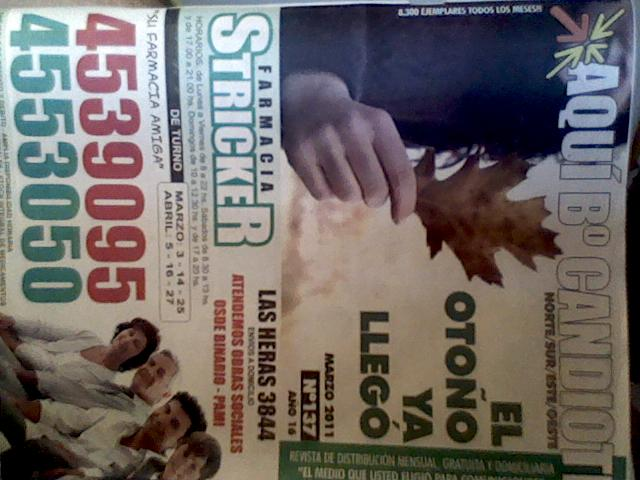
\includegraphics[width=2.5in]{../exp1/train_brillante_BH/train_brillante} \label{fig:train_brillante}}\\
\subfloat[][Imagen patrón con condición $B_{L}$.]{
\includegraphics[width=2.5in]{../exp1/train_oscura_BL/train_oscura} \label{fig:train_oscura}}
\caption[Imágenes obtenidas para condiciones de iluminación diferentes]{Imágenes obtenidas para condiciones de iluminación diferentes.}
\label{fig:prueba_iluminacion_realce_detalles_2_imagenes}
\end{figure}
 
Los resultados de las técnicas aplicadas con los parámetros que se mencionarán a continuación, pueden observarse en la Fig. \ref{fig:mejoras_iluminacion_normal_BN}, Fig. \ref{fig:mejoras_iluminacion_brillante_BH} y Fig. \ref{fig:mejoras_iluminacion_oscura_BL} para la condiciones de iluminación $B_{N}$, $B_{H}$ y $B_{L}$, respectivamente. Por cuestiones de brevedad, haremos referencia a las imágenes de la Fig. \ref{fig:mejoras_iluminacion_normal_BN} para la condición $B_{N}$, pero una interpretación similar se puede realizar para las demás condiciones. 

La imagen patrón que se utilizó en la condición $B_{N}$ se encuentra ilustrada en la Fig. \ref{fig:iluminacion_BN_original} y es sobre ésta que se aplican las diferentes técnicas mencionadas. Para la \textit{transformación logarítmica}, el valor $c$ se estableció en $1$ y el resultado de aplicar esta transformación, se puede observar en la Fig. \ref{fig:iluminacion_BN_logaritmica}. El resultado la \textit{ecualización} puede apreciarse en la Fig. \ref{fig:iluminacion_BN_ecualizacion}, mientras que en la Fig. \ref{fig:iluminacion_BN_pasaaltos}, se puede visualizar el resultado de un \textit{filtrado pasa altos} con el kernel:
\begin{equation}
\label{eq:kernel_pasaaltos}
\begin{bmatrix}
\quad0 & -1 & \quad0\\
-1 & \quad5 & -1\\
\quad0 & -1 & \quad0
\end{bmatrix}
\end{equation}

En lo que respecta al \textit{filtrado de alta potencia}, se estableció el valor $A=2$ para la expresión \eqref{eq:form_alta_potencia} y se utilizó un kernel de un filtro pasa altos de la forma:
\begin{equation}
\label{eq:kernel_altapotencia}
\begin{bmatrix}
-1 & -1 & -1\\
-1 & \quad8 & -1\\
-1 & -1 & -1
\end{bmatrix}
\end{equation}
El resultado de su aplicación se puede ver en la Fig. \ref{fig:iluminacion_BN_altapotencia}.

Finalmente, se propuso una alternativa mixta para aumentar el contraste de la imagen realzando a su vez los detalles. Para ello, se aplicó la \textit{ecualización del histograma} y posteriormente, sobre la imagen resultante, el \textit{filtrado de alta potencia} con los parámetros mencionados anteriormente (Fig. \ref{fig:iluminacion_BN_ecyaltapotencia}).
\begin{figure}
\centering
\subfloat[][Imagen patrón con Ilum. $B_{N}$]{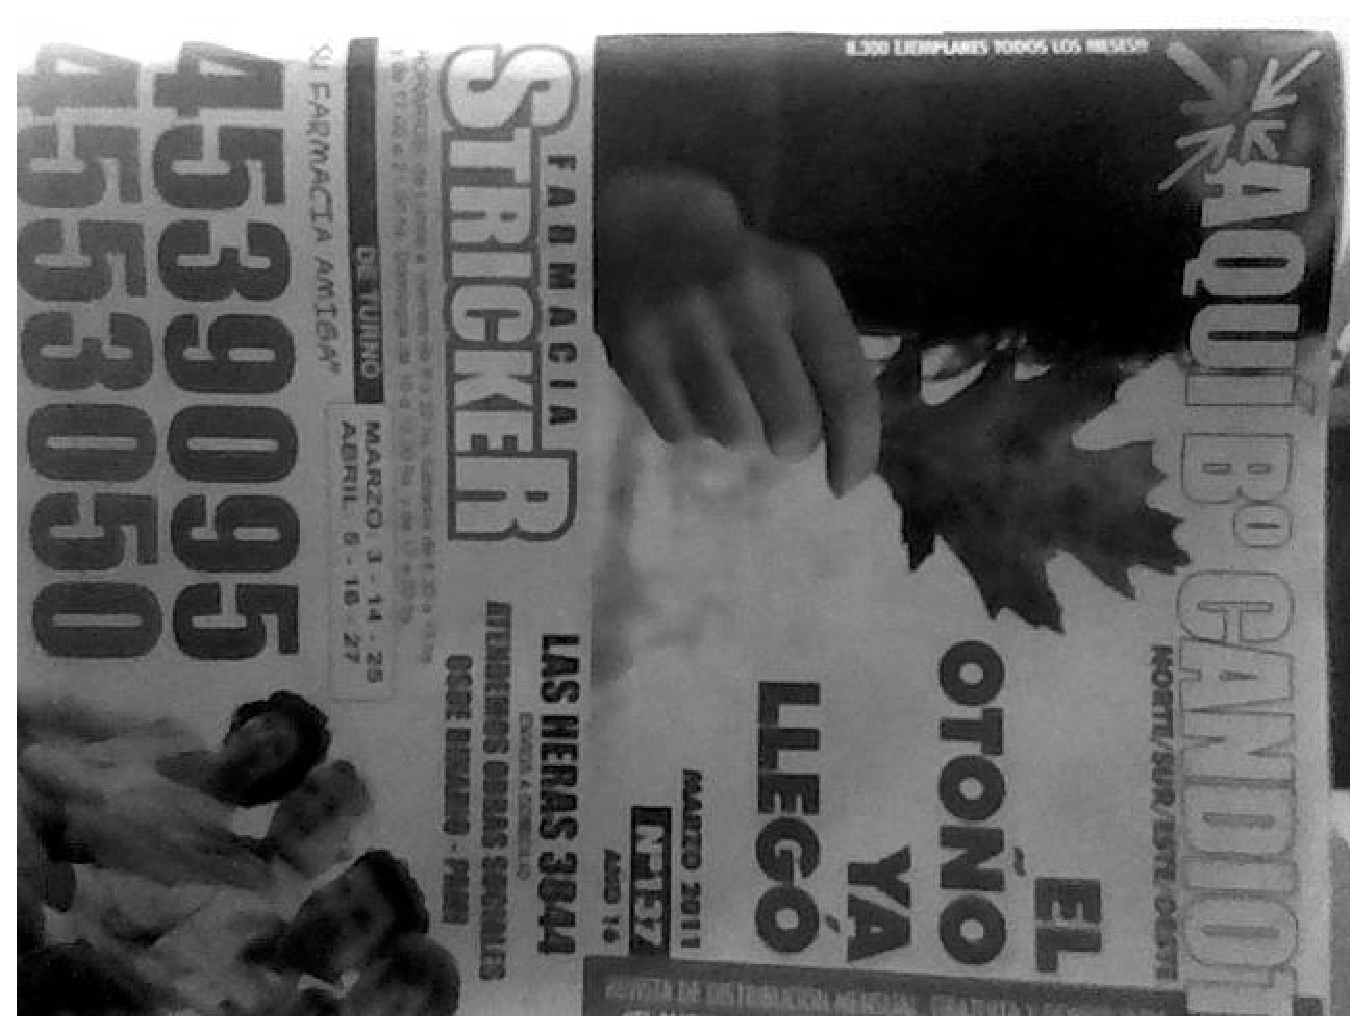
\includegraphics[width=2.5in]{../exp1/train_normal_BN/train_normal_grises} \label{fig:iluminacion_BN_original}}
\subfloat[][Transformación logarítmica]{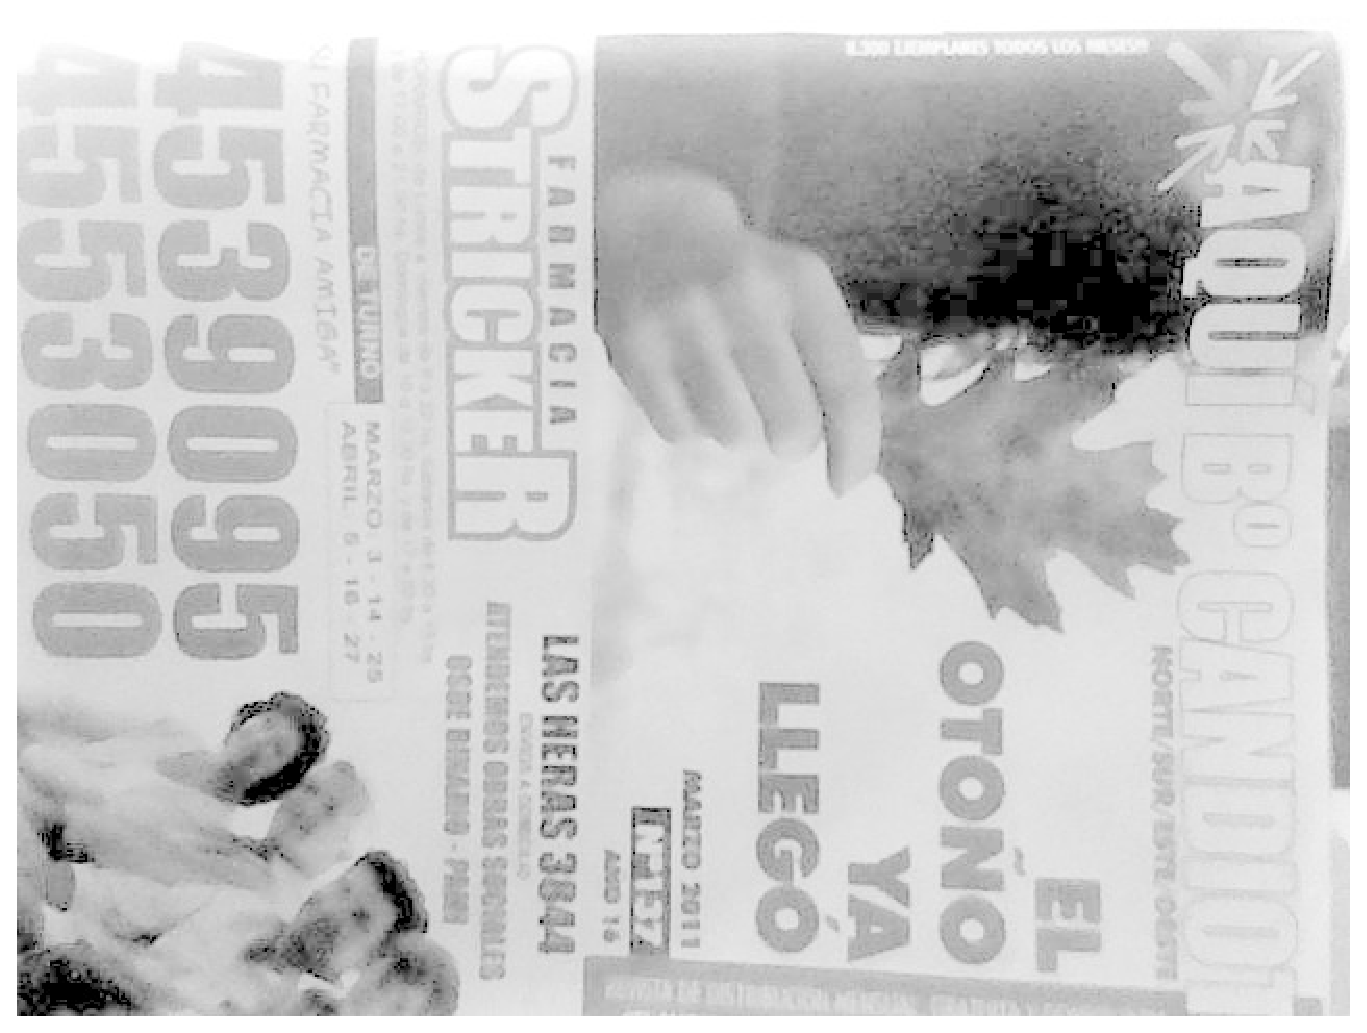
\includegraphics[width=2.5in]{../exp1/train_normal_BN/train_normal_515} \label{fig:iluminacion_BN_logaritmica}}\\
\subfloat[][Ecualización]{\includegraphics[width=2.5in]{../exp1/train_normal_BN/keypoints2} \label{fig:iluminacion_BN_ecualizacion}}
\subfloat[][Filtrado pasa altos]{\includegraphics[width=2.5in]{../exp1/train_normal_BN/keypoints3} \label{fig:iluminacion_BN_pasaaltos}}\\
\subfloat[][Filtrado de alta potencia]{\includegraphics[width=2.5in]{../exp1/train_normal_BN/keypoints4} \label{fig:iluminacion_BN_altapotencia}}
\subfloat[][Ecualización + filtrado de alta potencia]{\includegraphics[width=2.5in]{../exp1/train_normal_BN/keypoints5} \label{fig:iluminacion_BN_ecyaltapotencia}}\\
\caption[Resultados de aplicar las técnicas para la mejora en iluminación y detalles en condición $B_{N}$]{Resultados de aplicar las técnicas para la mejora en iluminación y detalles en condición $B_{N}$.}
\label{fig:mejoras_iluminacion_normal_BN}               %% Etiqueta para la figura entera
\end{figure}
%%%%%%%%%%%%%%%%%%%%%%%%%%%%%%%%%%%%%%%%%%%%%%%%%%%%%%%%%%%%%%%%%%%%%%%%%%%%%%%%%%%%%%%%%%%%%%%%%%%
\begin{figure}
\centering
\subfloat[][Imagen patrón con Ilum. $B_{H}$]{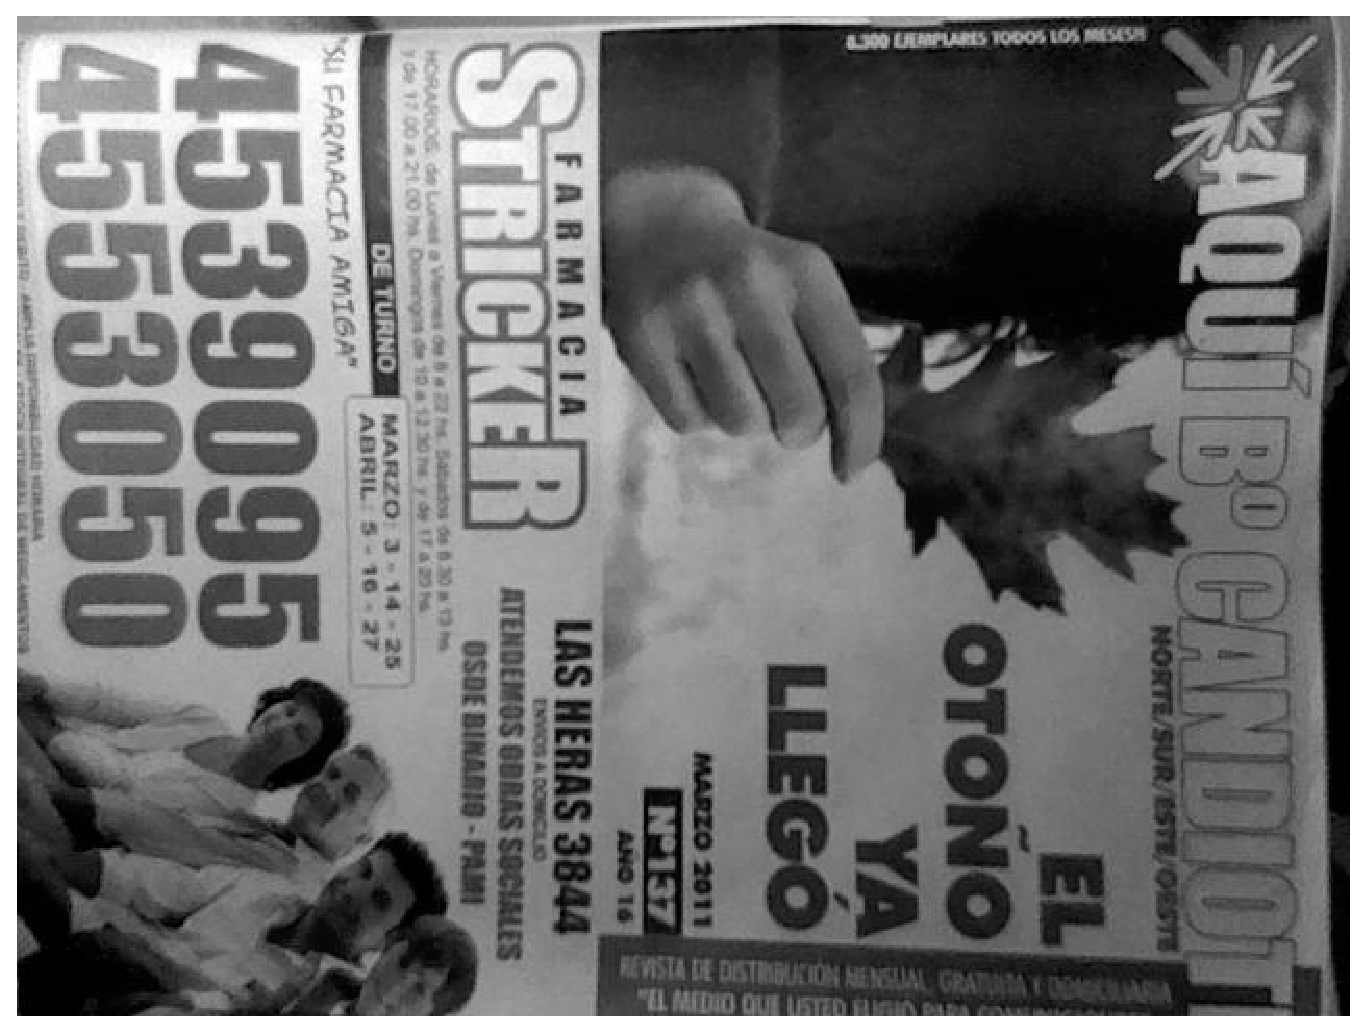
\includegraphics[width=2.5in]{../exp1/train_brillante_BH/train_brillante_grises} \label{fig:iluminacion_BH_original}}
\subfloat[][Transformación logarítmica]{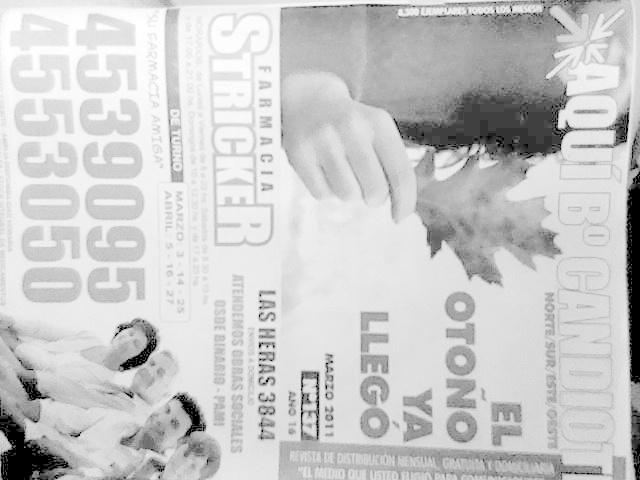
\includegraphics[width=2.5in]{../exp1/train_brillante_BH/train_brillante622} \label{fig:iluminacion_BH_logaritmica}}\\
\subfloat[][Ecualización]{\includegraphics[width=2.5in]{../exp1/train_brillante_BH/keypoints2} \label{fig:iluminacion_BH_ecualizacion}}
\subfloat[][Filtrado pasa altos]{\includegraphics[width=2.5in]{../exp1/train_brillante_BH/keypoints3} \label{fig:iluminacion_BH_pasaaltos}}\\
\subfloat[][Filtrado de alta potencia]{\includegraphics[width=2.5in]{../exp1/train_brillante_BH/keypoints4} \label{fig:iluminacion_BH_altapotencia}}
\subfloat[][Ecualización + filtrado de alta potencia]{\includegraphics[width=2.5in]{../exp1/train_brillante_BH/keypoints5} \label{fig:iluminacion_BH_ecyaltapotencia}}\\
\caption[Resultados de aplicar las técnicas para la mejora en iluminación y detalles en condición $B_{H}$]{Resultados de aplicar las técnicas para la mejora en iluminación y detalles en condición $B_{H}$}
\label{fig:mejoras_iluminacion_brillante_BH}               %% Etiqueta para la figura entera
\end{figure}
%%%%%%%%%%%%%%%%%%%%%%%%%%%%%%%%%%%%%%%%%%%%%%%%%%%%%%%%%%%%%%%%%%%%%%%%%%%%%%%%%%%%%%%%%%%%%%%%%%%
\begin{figure}
\centering
\subfloat[][Imagen patrón con Ilum. $B_{L}$]{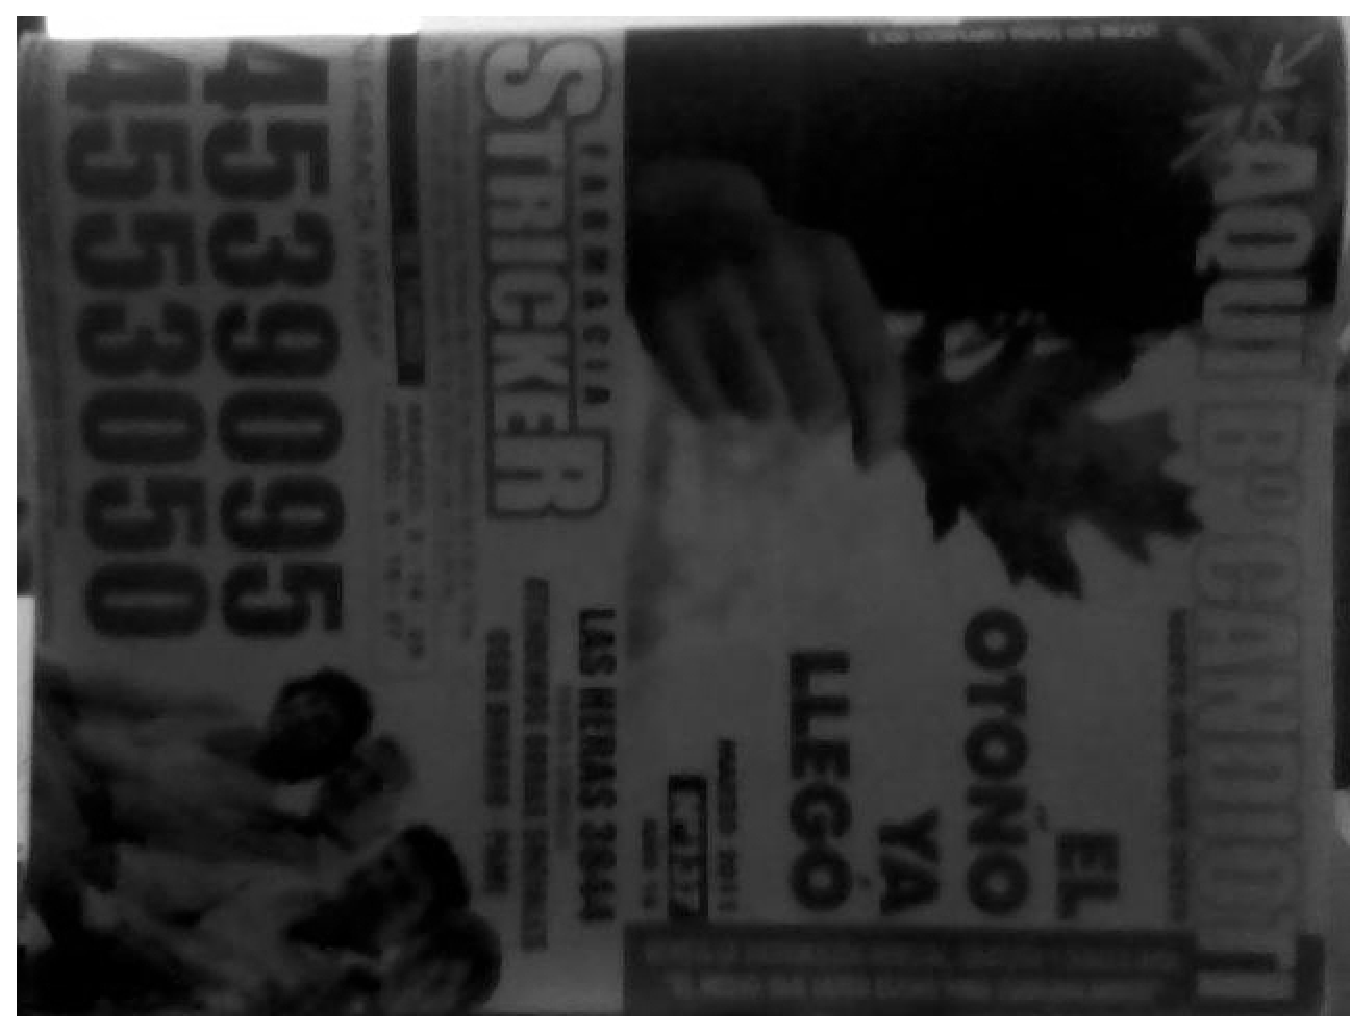
\includegraphics[width=2.5in]{../exp1/train_oscura_BL/train_oscura_grises} \label{fig:iluminacion_BL_original}}
\subfloat[][Transformación logarítmica]{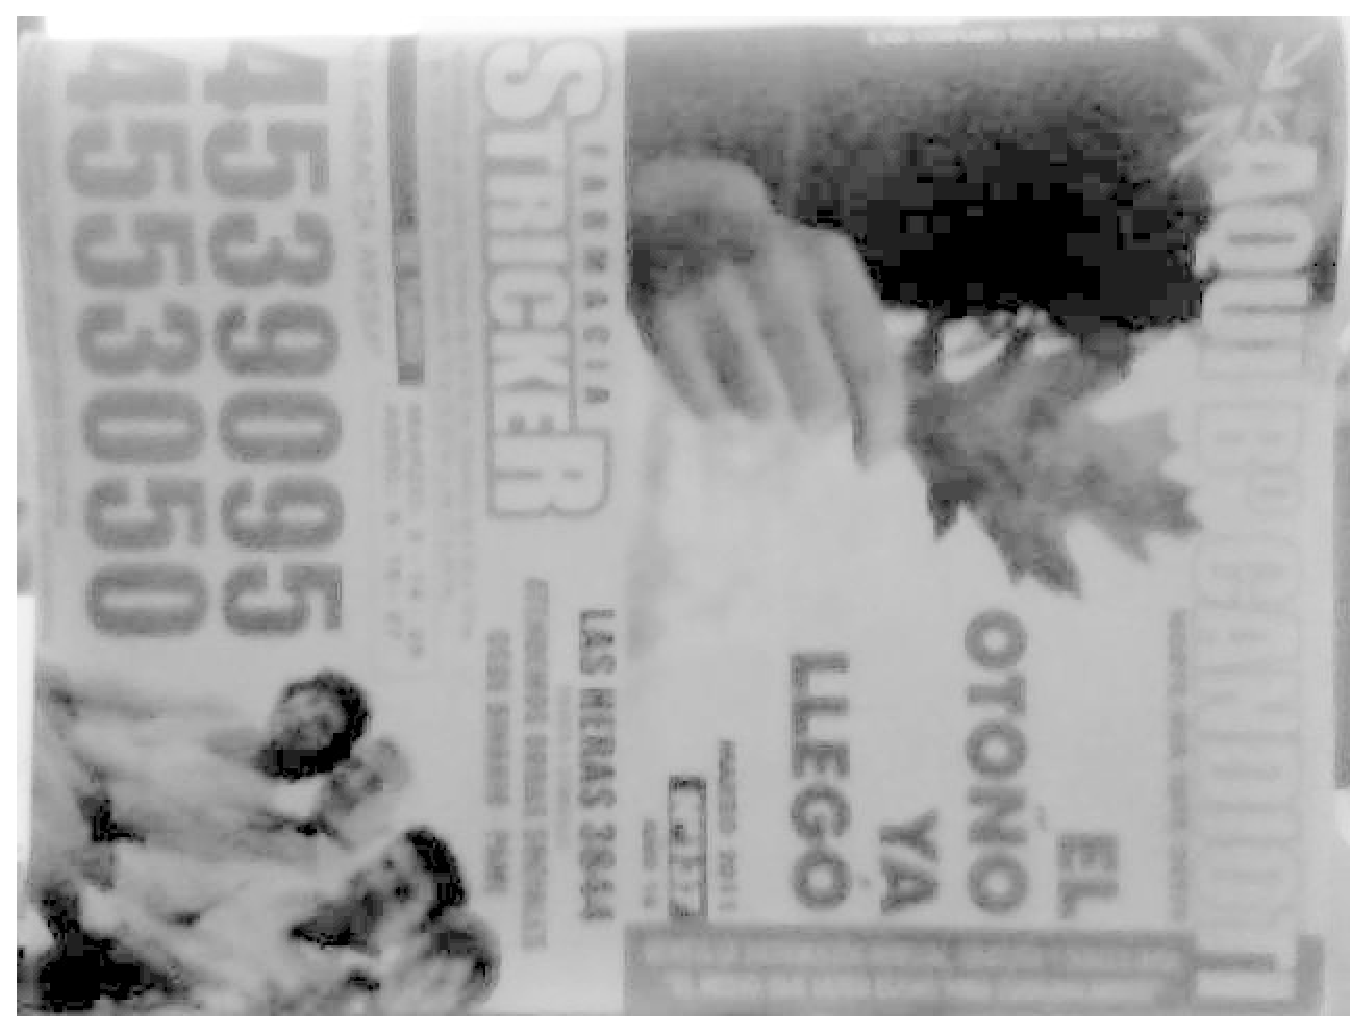
\includegraphics[width=2.5in]{../exp1/train_oscura_BL/train_oscura453} \label{fig:iluminacion_BL_logaritmica}}\\
\subfloat[][Ecualización]{\includegraphics[width=2.5in]{../exp1/train_oscura_BL/keypoints2} \label{fig:iluminacion_BL_ecualizacion}}
\subfloat[][Filtrado pasa altos]{\includegraphics[width=2.5in]{../exp1/train_oscura_BL/keypoints3} \label{fig:iluminacion_BL_pasaaltos}}\\
\subfloat[][Filtrado de alta potencia]{\includegraphics[width=2.5in]{../exp1/train_oscura_BL/keypoints4} \label{fig:iluminacion_BL_altapotencia}}
\subfloat[][Ecualización + filtrado de alta potencia]{\includegraphics[width=2.5in]{../exp1/train_oscura_BL/keypoints5} \label{fig:iluminacion_BL_ecyaltapotencia}}\\
\caption[Resultados de aplicar las técnicas para la mejora en iluminación y detalles en condición $B_{L}$]{Resultados de aplicar las técnicas para la mejora en iluminación y detalles en condición $B_{L}$}
\label{fig:mejoras_iluminacion_oscura_BL}               %% Etiqueta para la figura entera
\end{figure}
%%%%%%%%%%%%%%%%%%%%%%%%%%%%%%%%%%%%%%%%%%%%%%%%%%%%%%%%%%%%%%%%%%%%%%%%%%%%%%%%%%%%%%%%%%%%%%%%%%%
%%%%%%%%%%%%%%%%%%%%%%%%%%%%%%%%%%%%%%%%%%%%%%%%%%%%%%%%%%%%%%%%%%%%%%%%%%%%%%%%%%%%%%%%%%%%%%%%%%%
%%%%%%%%%%%%%%%%%%%%%%%%%%%%%%%%%%%%%%%%%%%%%%%%%%%%%%%%%%%%%%%%%%%%%%%%%%%%%%%%%%%%%%
% \subsection[Evaluación de mejora en iluminación y realce de detalles]{Métrica sobre procesos de mejora de iluminación y realce de detalles}
%\label{sec:discucion_mejoras_iluminacion}

Como es de esperar, al realizar un análisis visual subjetivo de los resultados obtenidos al aplicar las diversas técnicas, se puede observar que para las tres condiciones de iluminación, el \textit{filtrado pasa altos} y el \textit{filtro de alta potencia} realzan los detalles, mientras que la \textit{ecualización} mejora el contraste. En el caso particular de la condición $B_{L}$, se puede decir que la \textit{ecualización} y la combinación de \textit{ecualización y filtrado de alta potencia} son las que logran los mejores resultados respecto de las demás técnicas, esto como consecuencia de la maximización del contraste en la imagen resultante de la operación de ecualización.
% Con el objetivo medir el tiempo de procesamiento y la cantidad de características detectadas para cada técnica descripta en la Sec. \ref{subsec:mejoras_iluminacion}, se procedió con la aplicación de las mismas sobre dos imágenes: una con condición  cuyos resultados, pueden observarse en la tabla \ref{tabla:tiempos_realce_iluminacion} y \ref{tabla:tiempos_realce_iluminacion_brillante} respectivamente. El valor de umbral hessiano utilizado para la detección de características fue de $700$ en ambos casos.
%%%%%%%%%%%%%
%%%%%%%%%%%%%

Los resultados del tiempo de procesamiento (expresado en milisegundos) y la cantidad de puntos claves detectados para cada técnica en las tres condiciones de iluminación, se presentan resumidos en el Cuadro \ref{tabla:tiempos_realce_iluminacion}. Para la detección de puntos claves en la imagen, se utilizó un umbral hessiano que se estableció empíricamente en $700$ y fue el mismo para las tres condiciones de iluminación.
%%%%%%%%%%%%%
%%%%%%%%%%%%%
\begin{table}[htbp]
\caption[Tiempo de procesamiento en milisegundos y cantidad de características sobre la imagen patrón en diferentes condiciones de iluminación]{Tiempo de procesamiento en milisegundos y cantidad de características sobre la imagen patrón en condiciones de iluminación $B_{N}$, $B_{H}$ y $B_{L}$.}
\begin{tabular}{|l|r|c|c|c|}
\hline
 %& \multicolumn{2}{c|}{\textbf{Iluminación Normal}} \\ \hline
 & \multicolumn{1}{c|}{\textbf{t [ms]}} & \textbf{$B_{N}$} & \textbf{$B_{H}$} & \textbf{$B_{L}$}\\ \hline
Sin Procesamiento & 0.00 &  958 & 1297 & 154\\ \hline
Logaritmo & 7.15 & 515 & 622 & 493\\ \hline
Ecualización & \textbf{0.70} & 1546 & 1472 & 1233\\ \hline
F. Pasa Altos & 1.26 &  1633 & 2006 & 269\\ \hline
F. Alta Potencia & 3.10 & 1952 & 2216 & 353\\ \hline
Ec.+F. Alta Potencia & 4.31 & \textbf{2704} & \textbf{2443} & \textbf{2002}\\ \hline
\end{tabular}
\label{tabla:tiempos_realce_iluminacion}
\end{table}
%
% \begin{table}[htbp]
% \caption[Tiempo de procesamiento en milisegundos, Representación porcentual del tiempo y Cant. de características detectadas sobre la imagen patrón en condiciones de iluminación alta para diferentes procesos]{Tiempo de procesamiento en milisegundos, Representación porcentual del tiempo y Cant. de características detectadas sobre la imagen patrón en condiciones de iluminación alta (Fig. \ref{fig:train_brillante}) para los procesos descriptos en la Sec. \ref{subsec:mejoras_iluminacion} }
% \begin{tabular}{|l|r|c|c|}
% \hline
%  & \multicolumn{ 3}{c|}{\textbf{Iluminación Alta}} \\ \hline
%  & \multicolumn{1}{c|}{\textbf{t [ms]}} & \textbf{\%} & \textbf{Cant. Caract.} \\ \hline
% \textbf{Sin Proc} & 0,00 & 0,00 &  \\ \hline
% \textbf{Logaritmo} & 7,15 & 43,19 & 950 \\ \hline
% \textbf{Ecualización} & 0,70 & 4,22 & 1472 \\ \hline
% \textbf{F. Pasa Altos} & 1,27 & 7,65 & 2006 \\ \hline
% \textbf{F. Alta Pot.} & 3,13 & 18,91 & 2216 \\ \hline
% \textbf{Ec.+F. Alta Pot.} & 4,31 & 26,04 & 2443 \\ \hline
% \end{tabular}
% \label{tabla:tiempos_realce_iluminacion_brillante}
% \end{table}
% \subsubsection{Discusión}

%%%%%%%%%%%%%
%%%%%%%%%%%%%
En el Cuadro \ref{tabla:tiempos_realce_iluminacion}, se puede observar que el tiempo de procesamiento consumido para la aplicación del \textit{logaritmo} es superior a los demás valores, lo cual puede resultar incomprensible por tratarse de una operación sencilla. Se cree que el tiempo de cálculo se ve afectado por la forma en que fue implementado en el código de la aplicación: por un lado se debe tener en cuenta que la operación de logaritmo de OpenCV implementa el logaritmo neperiano y no el logaritmo en base 10, por lo cual se hizo necesario realizar varias operaciones para obtener el resultado correcto; por otro lado, existen casos en los que se describe que la instalación y compilación de OpenCV con soporte para Intel IPP\footnote{\url{http://opencv.willowgarage.com/wiki/IPP}} podría ser una solución al inconveniente, lográndose tiempos de cálculo más acotados. Sin embargo y como la cantidad de puntos característicos detectados es menor que cuando no se aplica procesamiento alguno (exceptuando la imagen en condiciones $B_{L}$), no se le dio mayor importancia.
% 
% La función logaritmo de OpenCV recibe como entrada imágenes de 32 bits, por ello, se hizo necesario convertir las imágenes de entrada de nuestra aplicación (de 8 bits) y es en esta operación de conversión donde existen varios reportes sobre lentitud con la versión de la librería de OpenCV utilizada. 

Las técnicas que involucran una operación de convolución (\textit{filtro pasa altos}, \textit{filtro de alta potencia}) obtienen tiempos de procesamiento mayores que la \textit{ecualización de la imagen}. Además y como es de esperar, la combinación de \textit{ecualización y filtrado de alta potencia} resulta en un mayor tiempo de procesamiento que los anteriormente mencionados.
% \begin{figure}[tbhp]
%    \centering
%         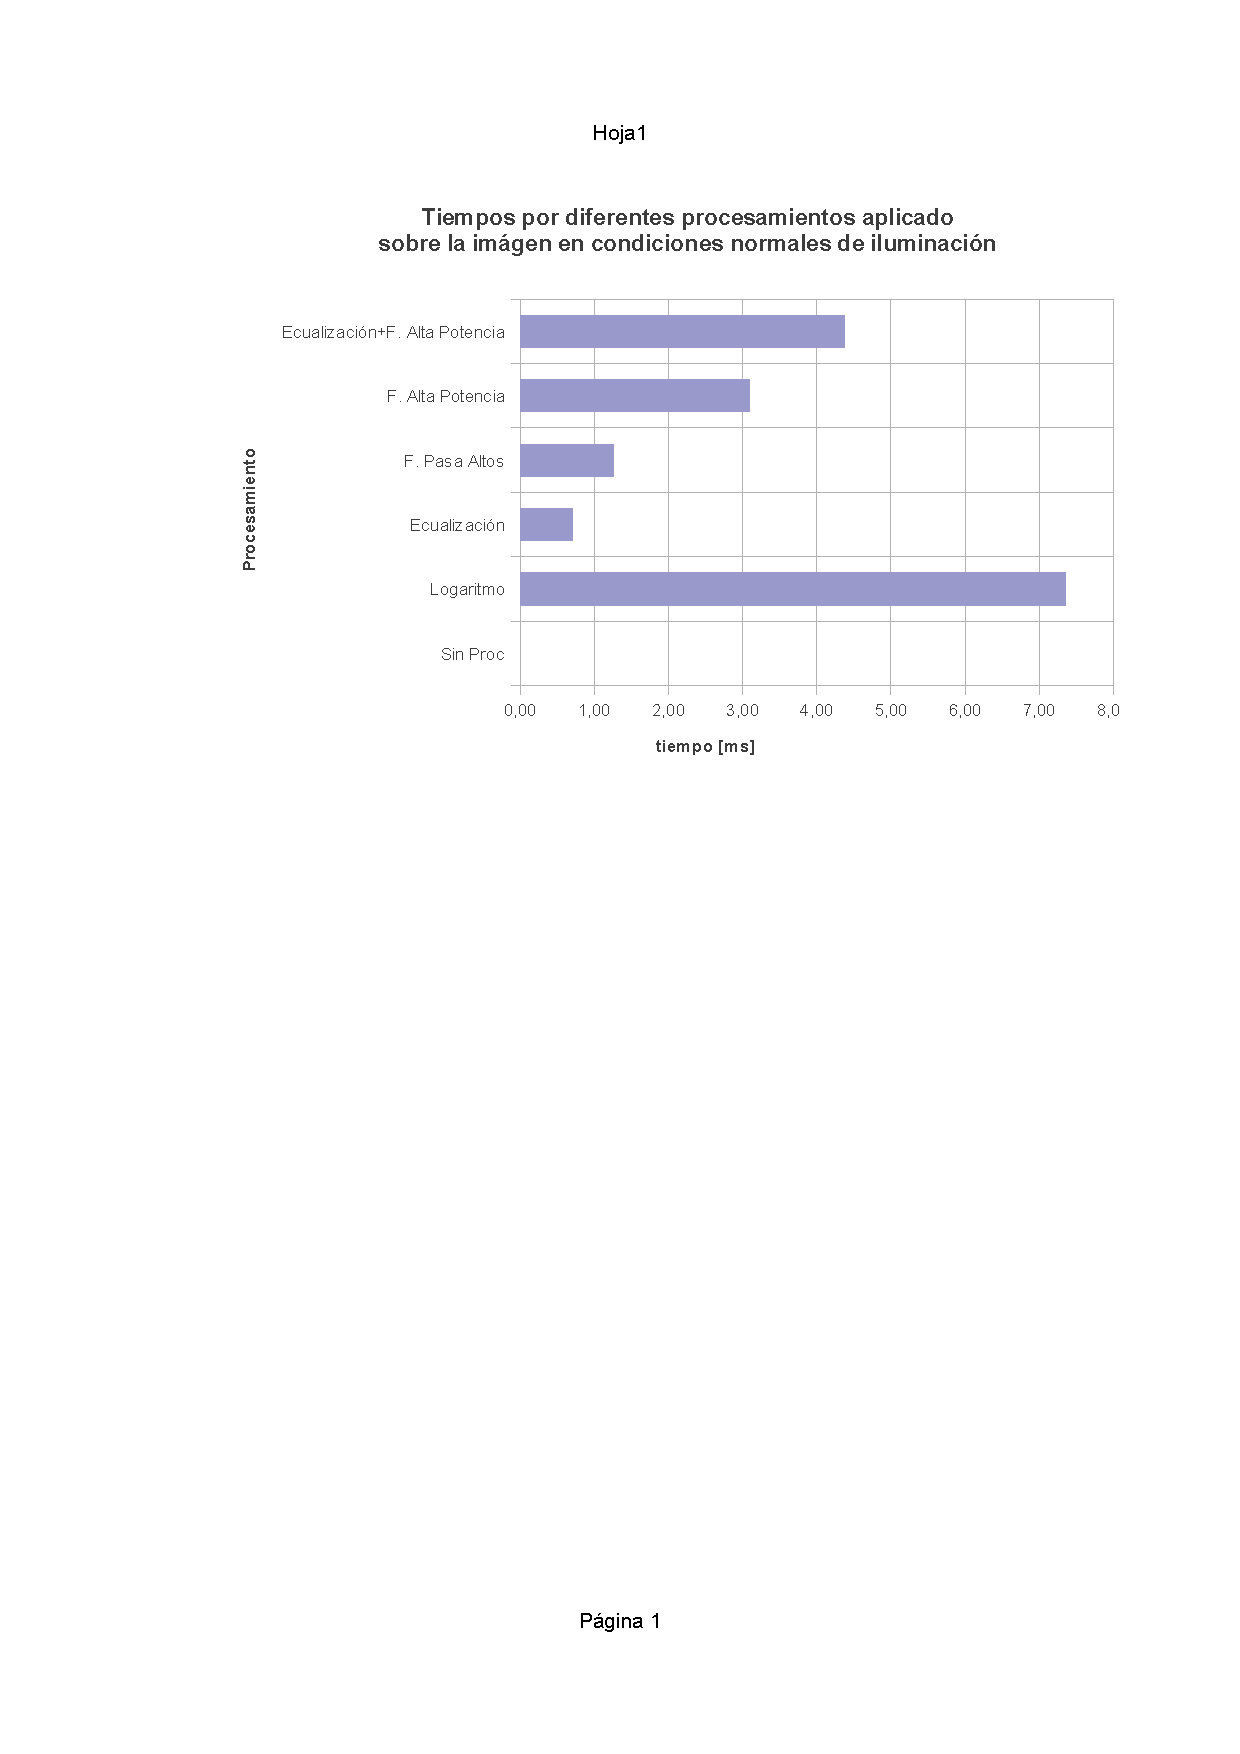
\includegraphics[scale=0.7]{../pruebas_modif/graph_tiempos_realces}
%     \caption[Comparación del rendimiento de los diferentes métodos utilizados en preproceso]{Tiempos para los diferentes procesamientos.%procesamientos de realce de detalles y mejora de iluminación aplicado sobre la imagen de la Fig. \ref{fig:train_normal} cuyos resultados están representados en la tabla \ref{tabla:tiempos_realce_iluminacion}
%     }
%    \label{graph:comparacion_tiempos}
% \end{figure}

% Si bien el gráfico representado en la Fig. \ref{tabla:tiempos_realce_iluminacion}, corresponde a la imagen obtenida bajo condiciones de iluminación normal, se puede observar un comportamiento similar para la imagen obtenida en condiciones de iluminación alta.

Si observamos en el Cuadro \ref{tabla:tiempos_realce_iluminacion} la cantidad de características detectadas para cada técnica, se aprecia que la combinación de \textit{ecualización + filtro de alta potencia} es la que presenta mayor cantidad de detecciones de puntos. Ésto es producto de una iluminación más uniforme lograda con la ecualización y del realce de los detalles como resultado de la aplicación del filtro de alta potencia.

Para el \textit{filtro pasa altos} y el de \textit{alta potencia} el incremento en la cantidad de puntos detectados se debe a que dichos filtros realzan las altas frecuencias y discontinuidades. También se puede notar que en el caso del \textit{filtrado de alta potencia}, se detectan más características que con el \textit{filtrado pasa altos} y ésto puede deberse a que el primero no afecta las bajas frecuencias. 
Mediante la \textit{ecualización}, se obtienen más puntos detectados que cuando no se procesa la imagen y si bien no supera a los otros procesamientos, ésta puede considerarse la más útil si la prioridad es el tiempo.

Del análisis realizado, se observa que todos los procesamientos aplicados incrementan la cantidad de puntos detectados, exceptuando el logaritmo (sólo incrementa la cantidad de puntos en la imagen en condiciones $B_{L}$). Se cree que la obtención de menor cantidad de puntos detectados como resultado de aplicar la transformación logarítmica en condiciones $B_{N}$ (Fig. \ref{fig:iluminacion_BN_logaritmica}) y $B_{H}$ (Fig. \ref{fig:iluminacion_BH_logaritmica}), se ve justificada en que las imágenes resultantes poseen intensidades más homogéneas obteniéndose menor distinción en los detalles. Para la condición $B_{L}$, la cantidad de puntos detectados se incrementa respecto al de la imagen sin procesamiento, como resultado de un aumento de los detalles (obsérvese el borde superior de la mano de la imagen en la Fig \ref{fig:iluminacion_BL_logaritmica} comparándose con la imagen de la Fig. \ref{fig:iluminacion_BL_original}).
\begin{figure}[tbhp]
   \centering
        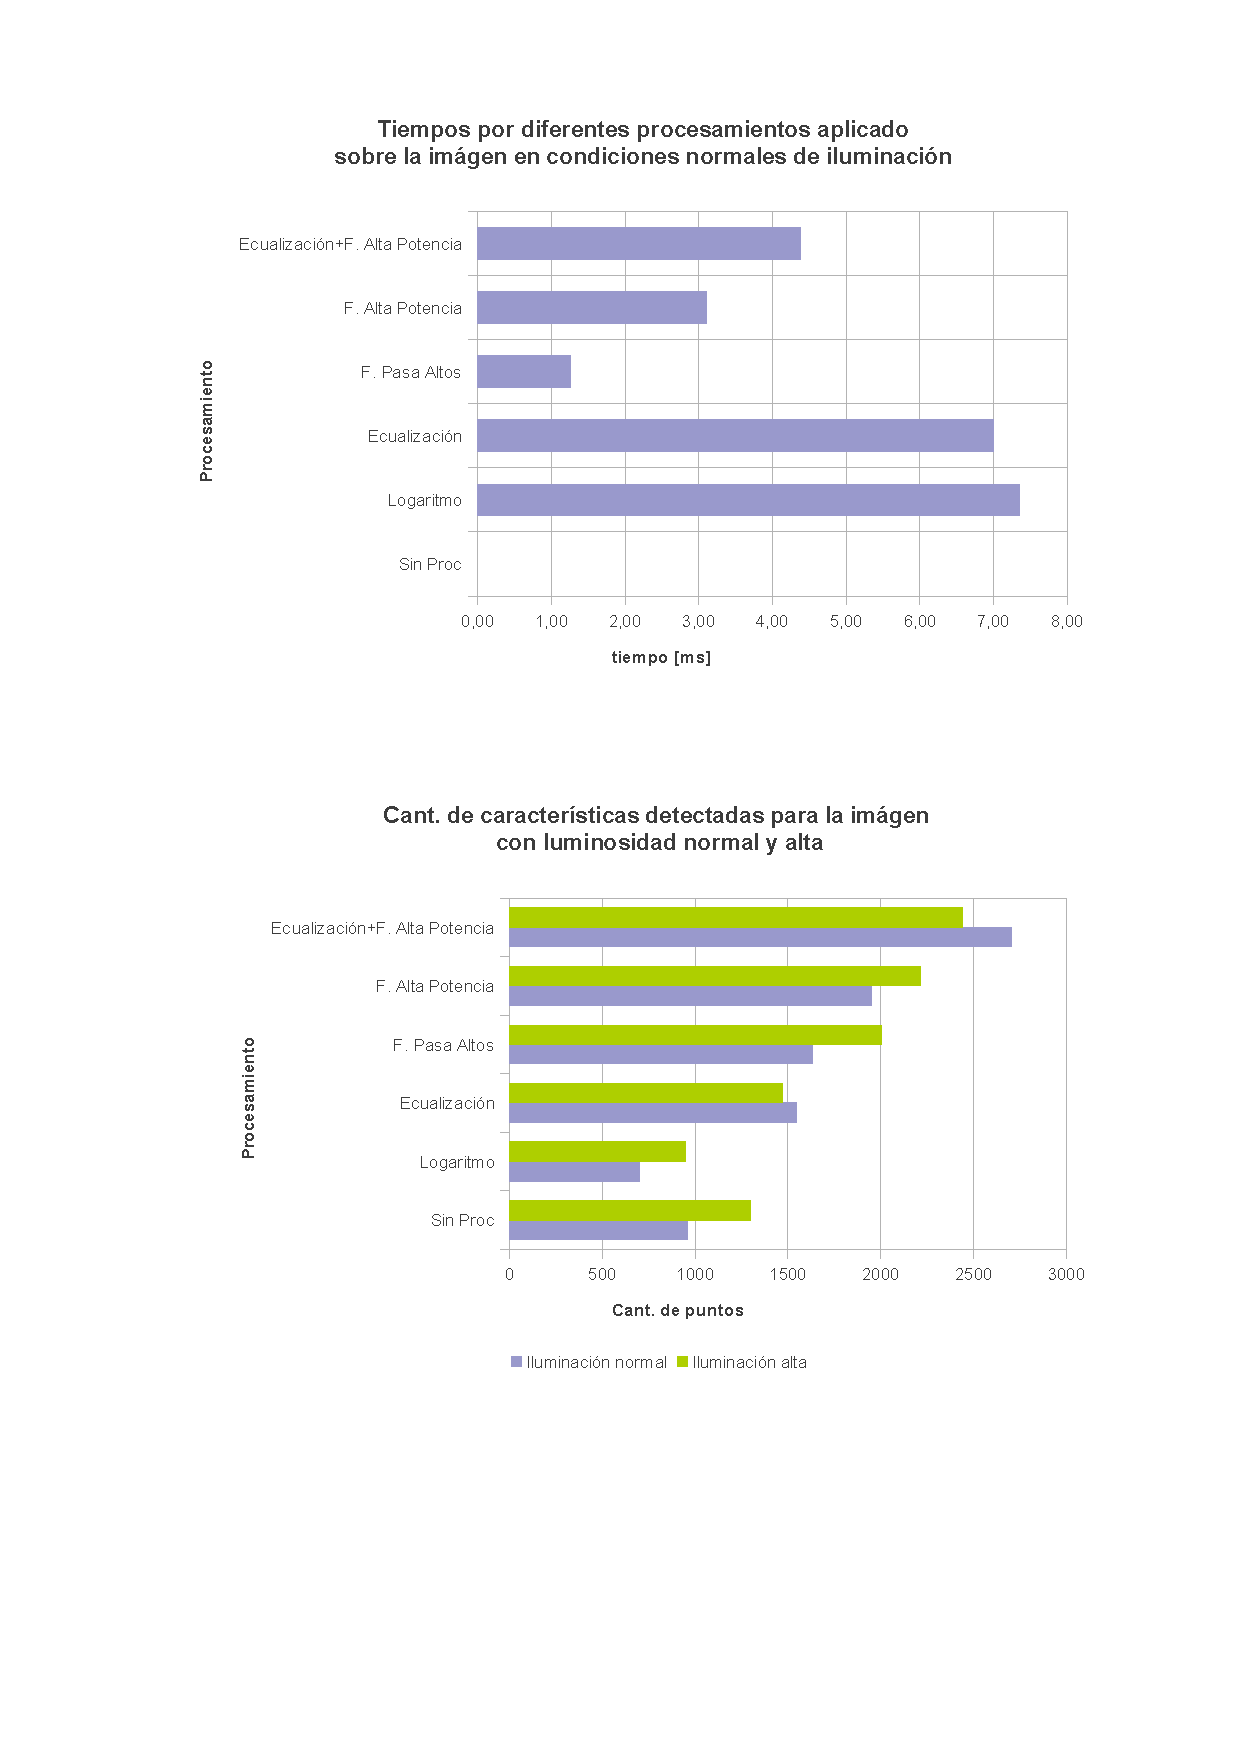
\includegraphics[scale=0.75]{../pruebas_modif/graph_ptos_realces}
    \caption[Cantidad de puntos detectados para la imagen con luminosidad normal, alta y baja]{Cantidad de puntos detectados para la imagen con luminosidad normal, alta y baja.}
   \label{graph:comparacion_cantptos}
\end{figure}

En el gráfico de la Fig. \ref{graph:comparacion_cantptos} se presenta una comparación de la cantidad de puntos detectados para las condiciones $B_{N}$, $B_{H}$ y$B_{L}$ establecidas. Claramente se advierte que cuando se realiza la combinación de \textit{ecualización y filtrado de alta potencia} en el caso de un ambiente en condición $B_{N}$, la cantidad de puntos detectados casi llega a triplicarse, respecto de cuando no se aplica técnica alguna. En tanto que en una condición $B_{H}$, la detección se duplica. Si analizamos lo que pasa en la condición de iluminación $B_{L}$, la cantidad de características posee valores bajos respecto de las otras condiciones de iluminación, ésta diferencia se evidencia aún más cuando no se aplica la ecualización, ya que los \textit{filtros pasa altos y de alta potencia} actúan sobre una imagen oscura sobre la que realzan los detalles, pero la diferencia de grises entre píxeles vecinos resulta insuficiente para una correcta detección.

Hasta aquí se han planteado tres condiciones ambientales diferentes. Además de éstas, se han realizado algunas pruebas adicionales tratando de observar el comportamiento del método en condiciones de iluminación intermedias (entre $B_{N}$, $B_{H}$ y $B_{L}$). Las mismas, no serán expuestas en este trabajo en detalle, sin embargo se realizará una reseña de las conclusiones obtenidas. 

Si bien la obtención de una mayor cantidad de características no presenta una garantía de lograr una mejor detección del objeto buscado (pueden ser características espurias), en la práctica y sobre todo en situaciones de iluminación baja o en una condición intermedia entre $B_{L}$ y $B_{N}$, donde la cantidad de características resulta insuficiente para lograr la detección del objeto, se notó que al aplicar \textit{ecualización} o \textit{ecualización + filtro de alta potencia}, se pudo detectar el objeto que previamente y sin procesamiento, no resultaba detectable. A pesar de obtener una correcta detección, se presentaron casos en que la detección fue ``intermitente''. Se varió el umbral hessiano de forma de discriminar menos puntos característicos, pero no se obtuvieron resultados apreciablemente superiores.

En lo que respecta a las condiciones $B_{N}$ y $B_{H}$, los resultados obtenidos sin la aplicación de un procesamiento de mejora del realce de iluminación y detalles, resultaron satisfactorios en las mayorías de las pruebas. Si bien la aplicación de las técnicas de \textit{ecualización}, \textit{filtrado pasa altos}, \textit{filtrado de alta potencia} y la combinación de \textit{ecualización y filtrado de alta potencia} mejoran la detección incrementando las características halladas y la robustez general del método, esto repercute negativamente en el tiempo de procesamiento, sobre todo en la aplicación de la \textit{ecualización} y la combinación con el \textit{filtro de alta potencia}. Sin embargo, la aplicación de estas técnicas cuando se está en presencia de un ambiente de iluminación intermedio entre $B_{L}$ y $B_{N}$, contribuyen a incrementar la calidad en la detección. En la práctica las decisiones dependerán de lo que se quiera priorizar (calidad en la detección o velocidad de ejecución) y del ambiente en que se use el método. En base a ello, se puede tomar la decisión de la técnica a utilizar, como así también del umbral hessiano que permita la mejor relación entre velocidad y calidad de detección.
% \label{sec:pruebas_resultados_discucion}
% Se intentó descartar un fotograma en el procesado del método para acelerar los tiempos, pero el resultado fue ver un video ``con saltos''.
% El histograma de la imagen con iluminación normal se notaba más concentrando en ciertos valores de grises que el histograma sobre la condición de iluminación alta. El resultado de la ecualización para el primero resultó con valores más dispares que en el caso de la de iluminación alta (más plano).  cuanto más plano el histograma ??
%%%%%%%%%%%%%%%%%%%%%%%%%%%%%%%%%%%%%%%%%%%%%%%%%%%%%%%%%%%%%%%%%%%%%%%%%%%%%%%%%%%%%%%%%%%%%%%%%%%%%%%%%%
%%esto viene del paper original de SURF:
% \section{Resultados SURF}
% Para un estudio comparativo con otros detectores y descriptores, nos referiremos a \ref{Bay06surf:speeded}. SURF ya ha sido testeado en algunas aplicaciones reales. Para reconocimiento de objetos, su performance ha sido ilustrada en \ref{Bay06gool.interactive}. Tomando esta aplicación para la registración de imágenes, nos enfocaremos en este artículo en el problema más difícil de calibración de la cámara y reconstrucción 3D, también en casos de wide-baseline.
\subsection{Experimento 2}
En el capítulo \ref{c:parte4}, se ha descripto el diagrama de flujo del método desarrollado, el cual presenta condicionales que permiten mejorar la detección y minimizar los tiempos de procesamiento. En esta sección se analizan y discuten los tiempos que insumen los procesos observables en el diagrama de la Fig. \ref{fig:diagrama_metodo} para obtener una conclusión más detallada sobre la efectividad de las alternativas planteadas.

Cuando se realiza el procesamiento en condiciones de baja iluminación (como se ha descripto en la Sec. \ref{subsec:paraqumetros_utilizados}), la detección no resulta del todo estable (se produce efecto de ``parapadeo'' seguido y repetitivo del objeto de RA). Dado que aquí se desea obtener conclusiones cuando el método es ``estable'' en la detección, se realizaron dos pruebas en condiciones de iluminación $B_{N}$ y $B_{H}$, estableciéndose empíricamente el umbral hessiano para lograr un equilibrio entre el tiempo de procesamiento y la correcta detección del objeto. La aplicación de alguna de las técnicas mencionadas en el ``Pre-Procesamiento de Iluminación y Realce de detalles'' no fue necesaria, ya que con las condiciones ambientales se obtuvieron resultados aceptables. Si bien aplicar alguna de estas técnicas mejora la calidad de detección, también incrementa el tiempo de procesamiento y es por ello que se deja a criterio del usuario la decisión de aplicarlas, según lo considere necesario. Las pruebas se definieron como:
\begin{itemize}
 \item \textbf{Prueba 1 (P1)}: duración: 1:50 minutos, umbral hessiano: 3500. Imagen con condición $B_{N}$ Fig. \ref{fig:train_normal} \footnote{Video de la prueba: \url{http://youtu.be/E8uGptzdEiw}}
 \item \textbf{Prueba 2 (P2)}: duración: 1:35 minutos, umbral hessiano: 5000. Imagen con condición $B_{H}$ Fig. \ref{fig:train_brillante} \footnote{Video de la prueba: \url{http://youtu.be/Pkiub9ZXP4k}}
\end{itemize}
Cabe aclarar que \textbf{P1} y \textbf{P2} son dos pruebas independientes, en las que el objeto presenta movimientos parecidos aunque diferentes en las escenas.

Para cada ciclo de la fase de ejecución de cada prueba se computaron los siguientes datos:
\begin{itemize}
 \item Tiempo de \textit{detección de movimiento},
 \item Tiempo de \textit{extracción y descripción de las características en BR} *,
 \item Tiempo de \textit{búsqueda de correspondencias} *,
 \item Tiempo de \textit{estimación de la homografía} *,
 \item Tiempo de comprobación \textit{contorno convexo y vértices válidos} *,
 \item Tiempo de \textit{transformación perspectiva de la imagen de RA utilizando la homografía} *,
 \item Cuadros por segundo (FPS),
 \item Total de puntos detectados en la imagen patrón,
 \item Total de puntos detectados en la imagen objeto,
 \item Total de coincidencias potencialmente válidas.
\end{itemize}

Si se observa el diagrama del ``método propuesto'' en la Fig. \ref{fig:diagrama_metodo}, se notará que las operaciones marcadas con (*) pueden ignorarse si se cumple una determinada condición en el ciclo de ejecución, sin impedir que se realice el enriquecimiento de la realidad. Esto como consecuencia del buffer de transformaciones descripto en la sección \ref{subsubsec:presente_en_alguno_3_frames_previos}. Así, por ejemplo si la comprobación de contornos convexo y vértices válidos (\textit{CCVV}) no se cumple, entonces no se calcula la transformación perspectiva (\textit{TP});  o si la homografía no es detectada, luego, no se realiza la \textit{CCVV} y por ende tampoco la \textit{TP}; aún más, si no se detecta movimiento en al escena, entonces ninguno de los procesos anteriormente mencionados es ejecutado. Así, todos estos condicionales producen que el tiempo promedio de procesamiento en el método propuesto disminuya cuando alguna (o todas) las operaciones son ignoradas. Adicionalmente se ha definido un proceso que denominamos ``método estándar'' que comprende sólo las siguientes operaciones de la Fig. \ref{fig:diagrama_metodo}: captura del flujo de video, conversión a escala de grises, extracción y descripción de características (en toda la imagen), búsqueda de correspondencias, estimación de la homografía, transformación perspectiva del objeto virtual y enriquecimiento de la realidad.
% 
% Si se eliminan todoPara identificar esta situación la denominaremos con el término: ``Proceso con bifuración en condicionales (\textit{PCBC})''; en caso contrario se denominará ``Proceso sin bifuración en condicionales (\textit{PSBC})'' y sería equivalente al diagrama del método propuesto en la Fig. \ref{fig:diagrama_metodo}, realizando las operaciones independientemente de lo que suceda en la escena.
%ver sino es al reves... esta medio confuso...

En el gráfico de la Fig. \ref{graph:graph_tiempos_3500}, se pueden observar los tiempos promedios en la fase de ejecución para el método propuesto y el método estándar en P1. %PSC => procesa==1
Para analizar los datos, se calcularon los FPS promedio ($FPS_{prom}$) para el proceso de ejecución. De ello, se pudo advertir que el valor de $FPS_{prom}$ para el método estándar fue de $6.93$ FPS, mientras que para el propuesto fue de $28.35$ FPS, lo cual constituye una mejora notable en el tiempo de procesamiento. Dicho de otro modo, la lógica de los condicionales planteados para mejorar el tiempo de procesamiento y la detección del objeto evidencia un gran incremento en los $FPS_{prom}$ y esto se debe en gran parte a que evita el proceso de extracción y descripción de características (observar que la barra verde en el gráfico representa casi la mitad de tiempo sobre la barra violeta).

En lo que respecta a los tiempos en los diferentes procesos, se puede visualizar en la Fig. \ref{graph:graph_tiempos_3500} que la extracción y descripción de características es la que más tiempo requiere, a pesar de que se minimizó el procesamiento en un área de la imagen (BR) como se explicó en la Sec. \ref{sec:deteccion_cambiante_imagen}. Experimentalmente se comprobó que si el área BR en la que se extraen características es del 50\% de la imagen patrón de $640 \times 480$ píxeles, el tiempo de procesamiento representa aproximadamente un 42\% del tiempo total que se requiere para extraer las características en la totalidad de la imagen.

El segundo proceso que más tiempo consume es la estimación de la homografía por tratarse de un método iterativo que estima la matriz $H$ y refina las coincidencias. La transformación perspectiva que involucra una interpolación, ocupa el tercer lugar, seguida de la búsqueda de correspondencias, la detección de movimiento y finalmente, la CCVV que está compuesta de operaciones triviales.
%en realida des todo el método vs cuando se realiza sin bifurcaciones... ver->
\begin{figure}[tbhp]
   \centering
        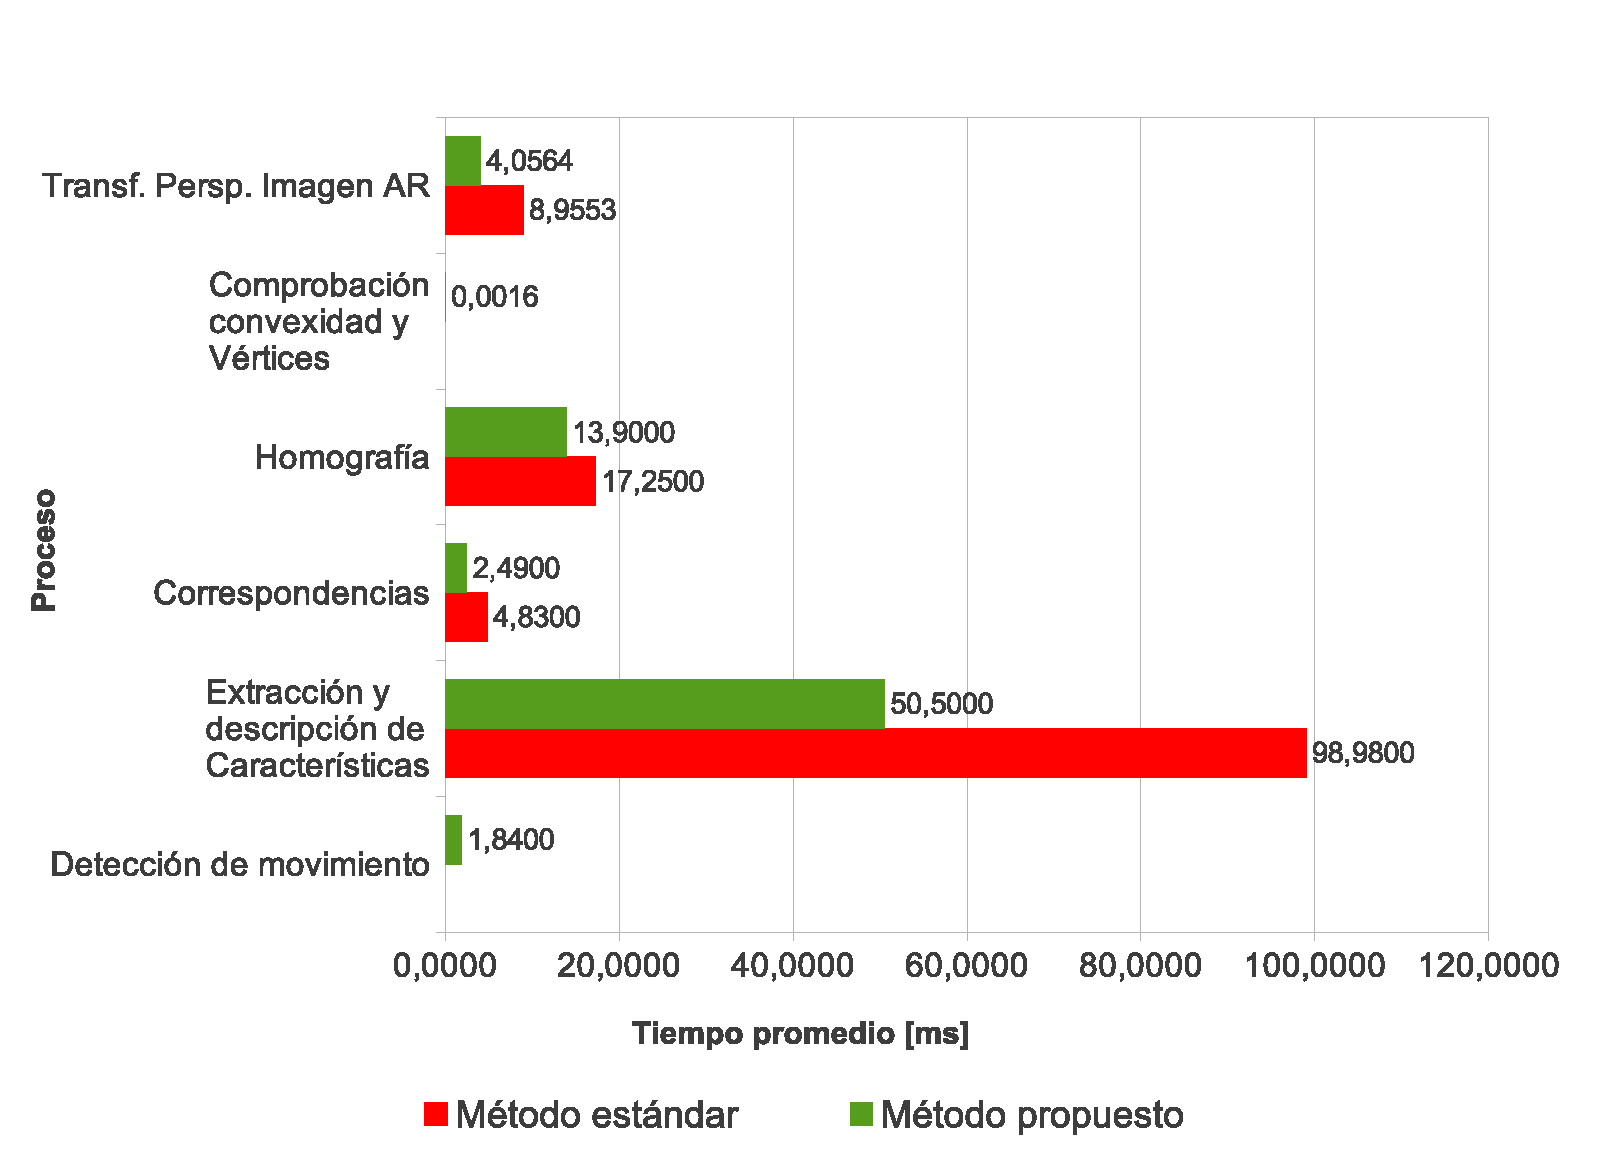
\includegraphics[scale=0.45]{../pruebas_modif/3500_sinproc/graph_tiempos_3500_presentacion1}
    \caption[Tiempos promedios de operación para los diferentes procesos en la Prueba 1]{Tiempos promedios de operación para los diferentes procesos en la Prueba 1}
   \label{graph:graph_tiempos_3500}
\end{figure}

En lo que respecta a total de puntos detectados y las potenciales correspondencias válidas, para P1 se detectaron 192 puntos claves en la imagen patrón y un promedio de 130 puntos en la imagen del flujo de video. De los mismos se obtuvo (en promedio) 38 pares de coincidencias potencialmente válidas, observándose un máximo de 81 pares.

En la Fig. \ref{fig:imagen_secuencia1_ejemplo} a \ref{fig:imagen_secuencia4_ejemplo} se presentan diferentes capturas del resultado final del método, utilizando como imagen patrón la Fig. \ref{fig:imagen_patron_ejemplo} y como objeto de realidad aumentada la imagen de la Fig. \ref{fig:imagen_objetoar_ejemplo}. El umbral hessiano se estableció a 3500 y la escena se encuentra en condición $B_{N}$ de iluminación.
\begin{figure}[tbhp]
\centering
\subfloat[][Imagen patrón con Ilum. $B_{N}$]{
\includegraphics[width=2.5in]{../pruebas_modif/capturas/usables/train_normal} \label{fig:imagen_patron_ejemplo}}
\subfloat[][Objeto de RA]{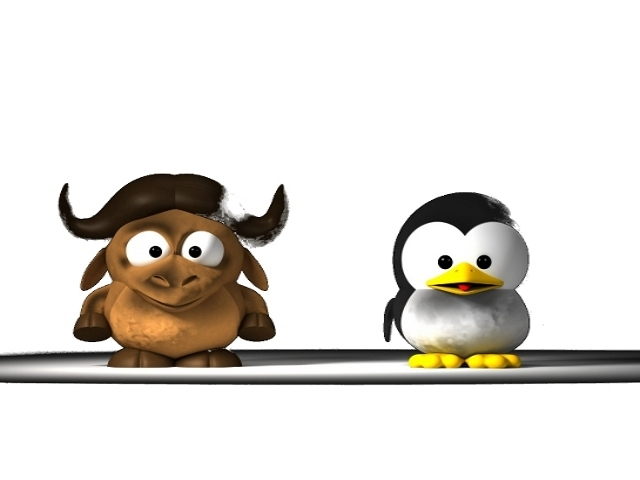
\includegraphics[width=2.5in]{../pruebas_modif/capturas/usables/pinguino} \label{fig:imagen_objetoar_ejemplo}}\\
\subfloat[][]{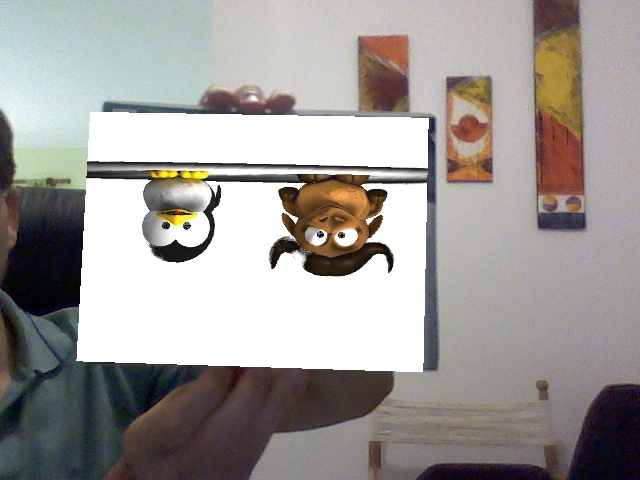
\includegraphics[width=2.5in]{../pruebas_modif/capturas/usables/captured154} \label{fig:imagen_secuencia1_ejemplo}}
\subfloat[][]{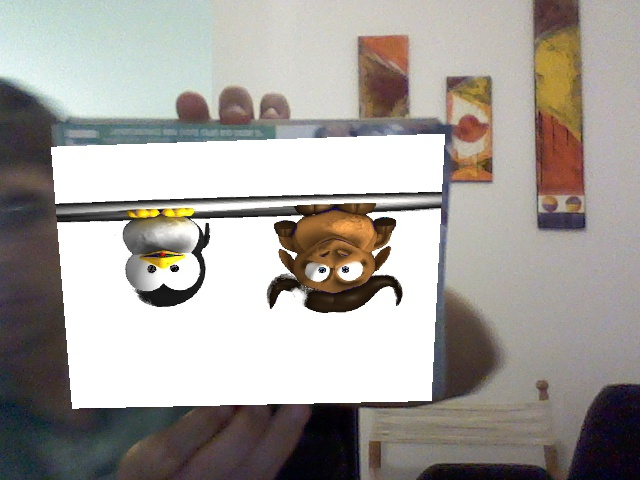
\includegraphics[width=2.5in]{../pruebas_modif/capturas/usables/captured135} \label{fig:imagen_secuencia2_ejemplo}}\\
\subfloat[][]{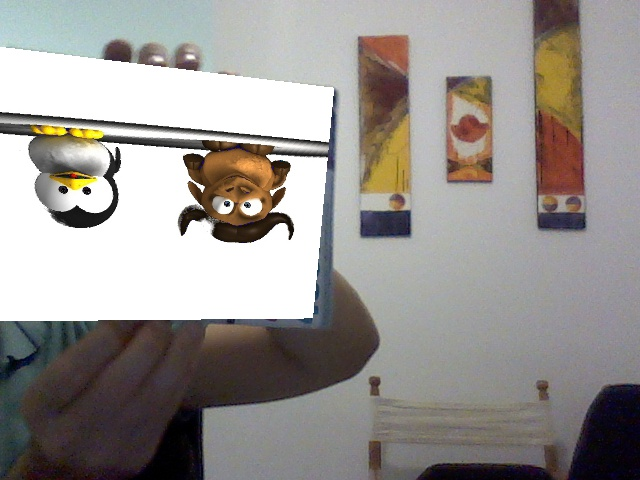
\includegraphics[width=2.5in]{../pruebas_modif/capturas/usables/captured141} \label{fig:imagen_secuencia3_ejemplo}}
\subfloat[][]{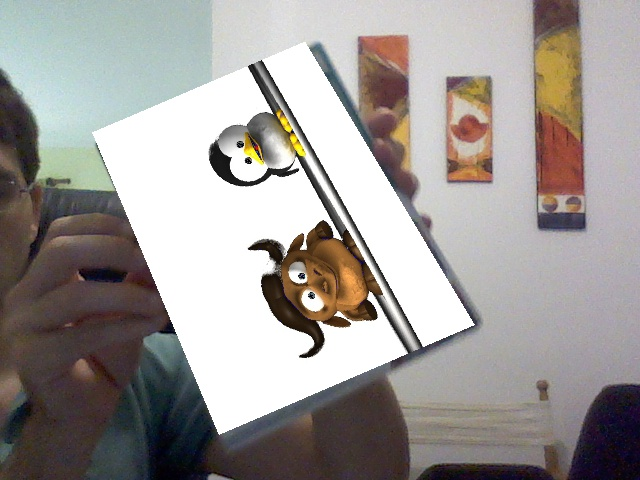
\includegraphics[width=2.5in]{../pruebas_modif/capturas/usables/captured207} \label{fig:imagen_secuencia4_ejemplo}}\\
\caption[Capturas de imágenes con enriquecimiento de la realidad]{Imagen patrón, objeto de RA y capturas de imágenes con enriquecimiento de la realidad.}
\label{fig:secuencia_ejemplo_BN}               %% Etiqueta para la figura entera
\end{figure}

% y si lo saco a lo de P2???? no tiene mucho sentido aca... quizás para mostrarlo sirve pero no para ponerlo acá....
En lo que respecta a la prueba P2, los detalles de los resultados no serán expuestos aquí para no extender este informe. Sin embargo, se debe mencionar que de su análisis se obtuvieron resultados similares en los órdenes de magnitud de tiempos por procesos. La cantidad de puntos claves detectados, no puede ser comparada con P1, ya que se trata de un umbral e imagen diferente, en condiciones diferentes de iluminación. De todas formas, podemos decir que la cantidad de puntos detectados en la imagen patrón, se vio incrementada a pesar de aumentar el umbral hessiano, debido a que la imagen sobre la cual se aplicó poseía mayor luminosidad y, por lo tanto mayores detalles apreciables.
%Para mayor detalle y análisis se deja un archivo digital adjunto con el presente trabajo con datos para $P2$ donde se puede corroborar lo aquí descripto.
%%%%%%%%%%%%%%%%%%%%%%%%%%%%%%%%%%%%%%%%%%%%%%%%%%%%%%%%%%%%%%%%%%%%%%%%%%%%%%%%%%%%%%%%%%%%%%%%%%%%%%%%%%%%%%%%%%%%%%%%%%%%%%%%%%%%%%%%%%%%%%%%%%%%
\section{Implementación de prototipos}
Como se ha mencionado en los objetivos específicos del presente trabajo, se ha propuesto implementar un prototipo que otorgue una visión del resultado final del método desarrollado. Para ello, se plantearon dos alternativas: en la primera de ellas, se enriquece la realidad mediante una imagen sobre la tapa de una revista y en la Fig. \ref{fig:secuencia_ejemplo_BN} se pueden ver algunas imágenes de esta implementación.

Como segunda alternativa, se planteó proveer información inherente a un producto comestible de forma publicitaria, en el que se brinda su precio y una imagen de un plato preparado con el mismo. El resultado del prototipo se puede visualizar en la secuencia de imágenes de la Fig. \ref{fig:ejemplos_protitipos}, donde: la Fig. \ref{fig:prototipo_img_detect} es la imagen patrón, la Fig. \ref{fig:protitpo_img_ar} es el objeto de realidad aumentada a sobreimprimir (el fondo blanco en la imagen es transparente) y las imágenes de la Fig. \ref{fig:first_detect_protitpo} a la Fig. \ref{fig:last_detect_prototipo}, representan diferentes capturas de la secuencia de video en la etapa de ejecución. Cabe aclarar que se presentan sólo algunas de las detecciones exitosas. Un video de este prototipo en condición $B_{N}$ de iluminación puede ser visto en la url: \url{http://youtu.be/j1xPZkglJHs}.
% Los prototipos fueron llevados a cabo en un ambiente de iluminación normal, sin procesamiento alguno para mejora de iluminación y detalles. => aclarar porqué.....

Los prototipos de realidad aumentada desarrollados aquí son sólo algunas de las aplicaciones posibles, y se pueden pensar en aplicaciones más avanzadas, como por ejemplo que provean una interactividad mayor con el usuario, a partir de la introducción de audio, videos, animaciones, etc.
\begin{figure}
\centering
\subfloat[][]{
\includegraphics[width=2.5in]{../imgvitina/vitina}\label{fig:prototipo_img_detect}}
\subfloat[][]{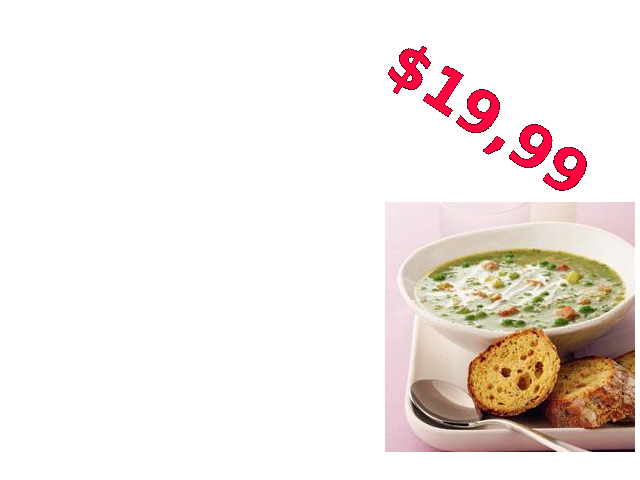
\includegraphics[width=2.5in]{../imgvitina/preciosvirtuales}\label{fig:protitpo_img_ar}}\\
% \subfloat[][]{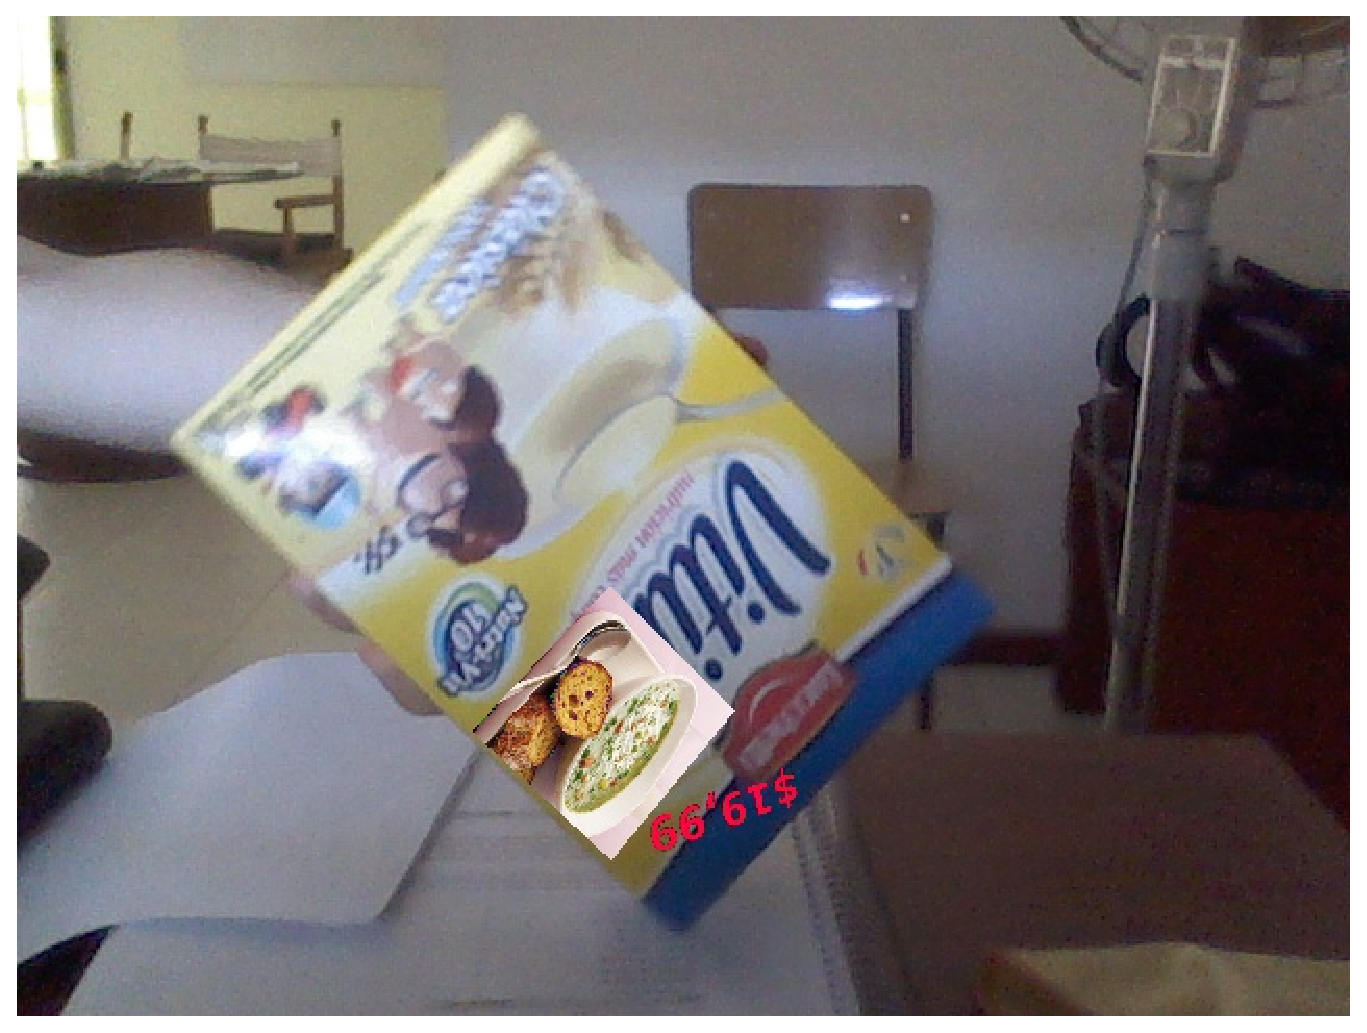
\includegraphics[width=2.5in]{../imgvitina/captured64,000000}\label{fig:first_detect_prototipo}}
% \subfloat[][]{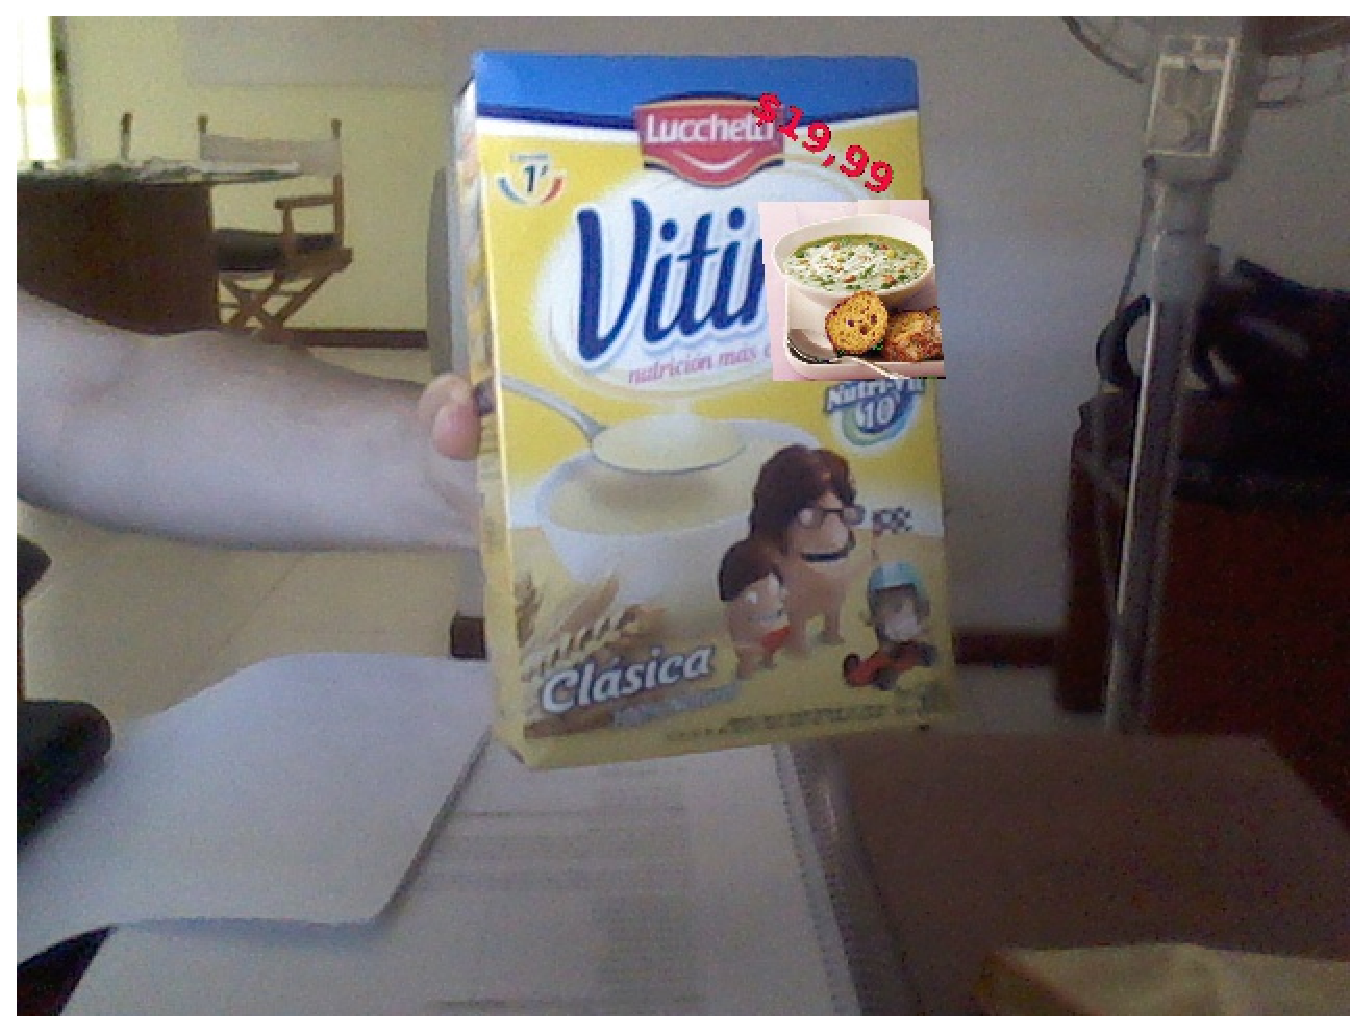
\includegraphics[width=2.5in]{../imgvitina/captured72,000000}}
\subfloat[][]{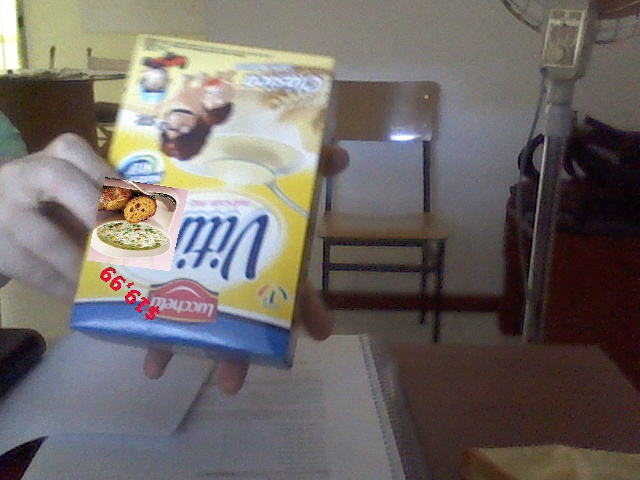
\includegraphics[width=2.5in]{../imgvitina/captured87,000000}\label{fig:first_detect_protitpo}} 
\subfloat[][]{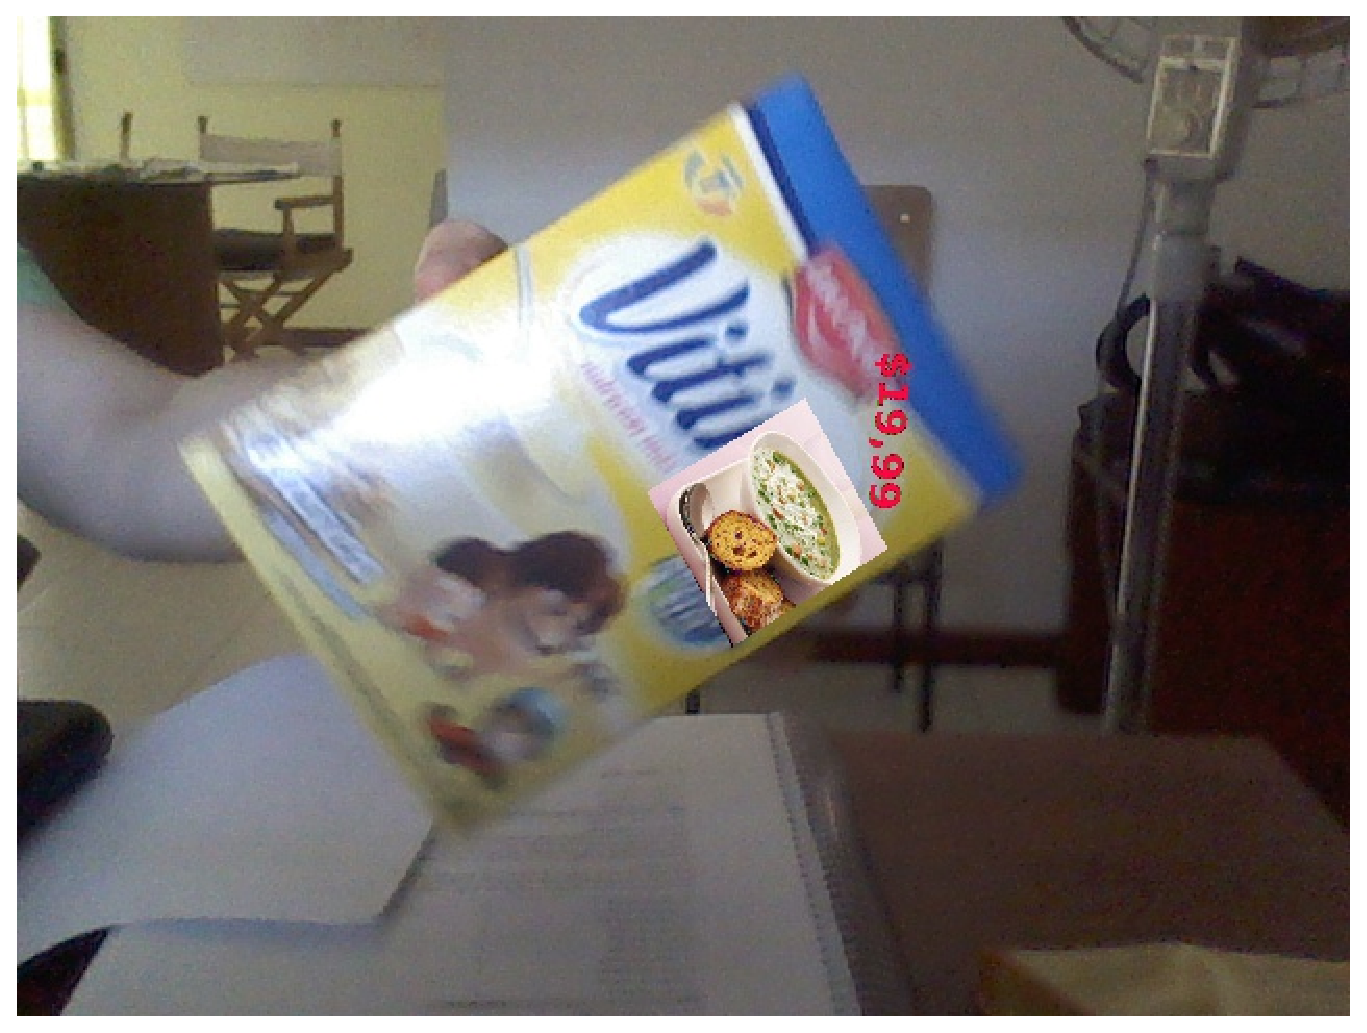
\includegraphics[width=2.5in]{../imgvitina/captured94,000000}}\\
% \subfloat[][]{
\includegraphics[width=2.5in]{../imgvitina/captured97,000000}}
% \subfloat[][]{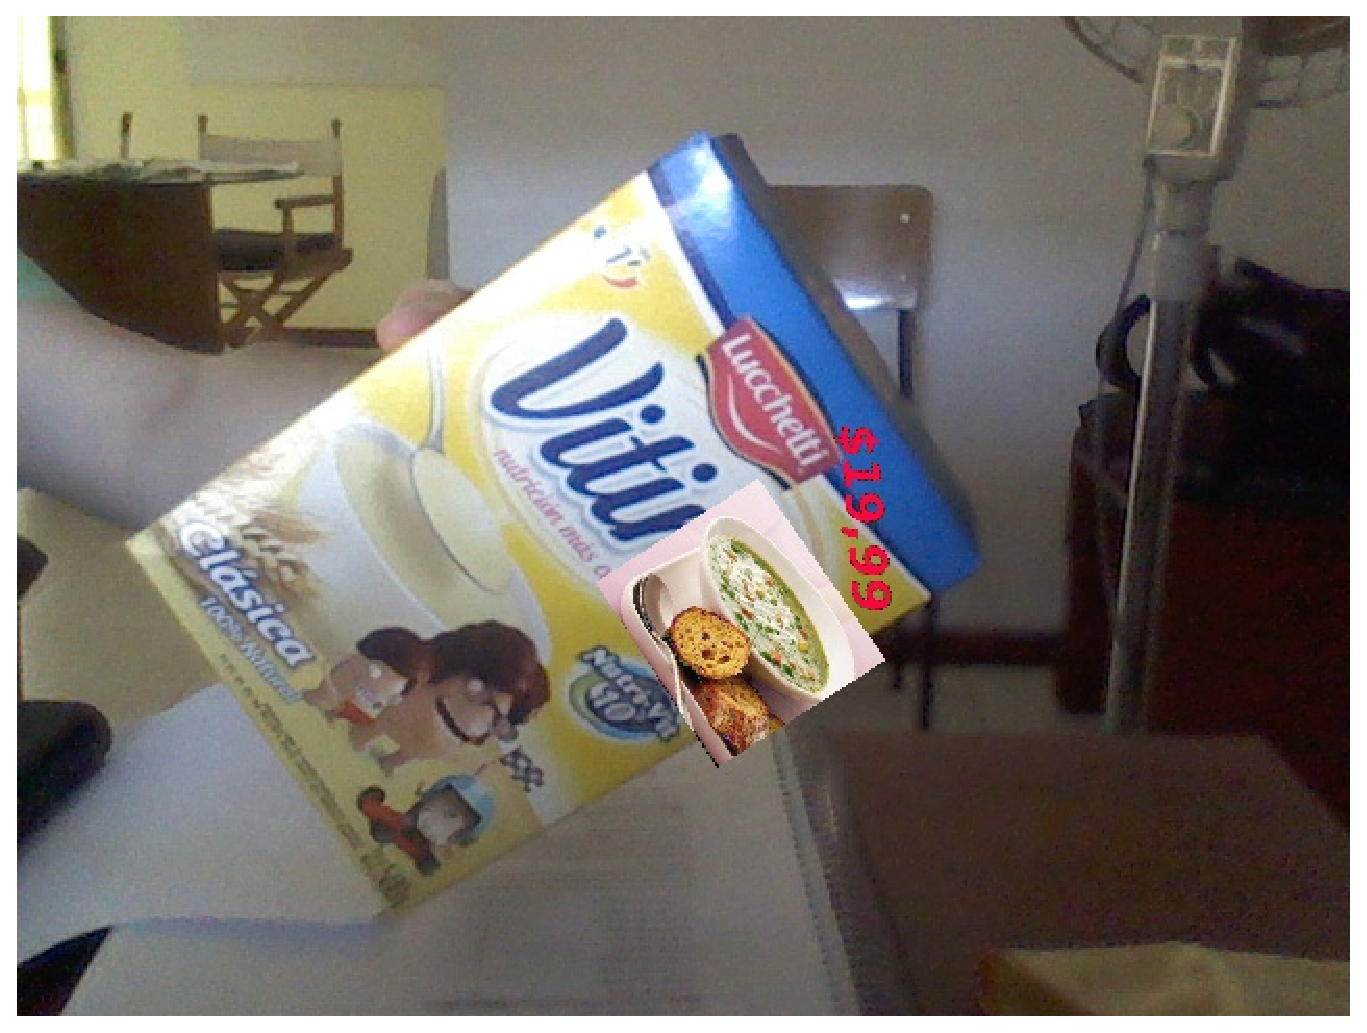
\includegraphics[width=2.5in]{../imgvitina/captured120,000000}}
% \subfloat[][]{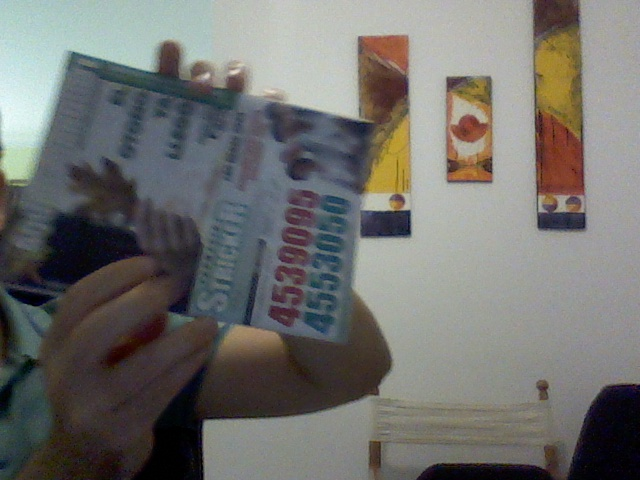
\includegraphics[width=2.5in]{../imgvitina/captured140,000000}}\\
\subfloat[][]{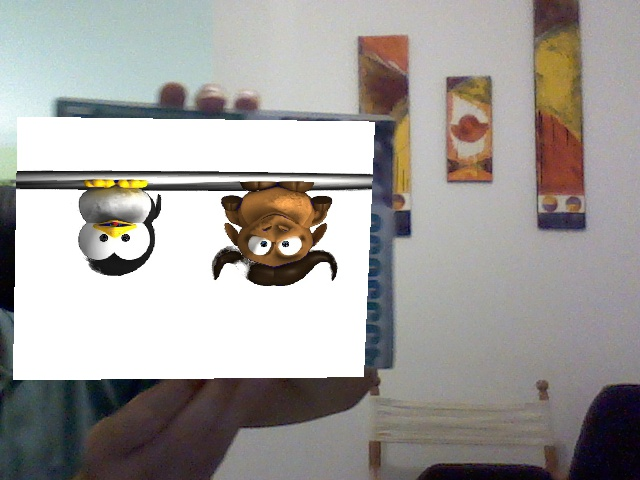
\includegraphics[width=2.5in]{../imgvitina/captured146,000000}}
% \subfloat[][]{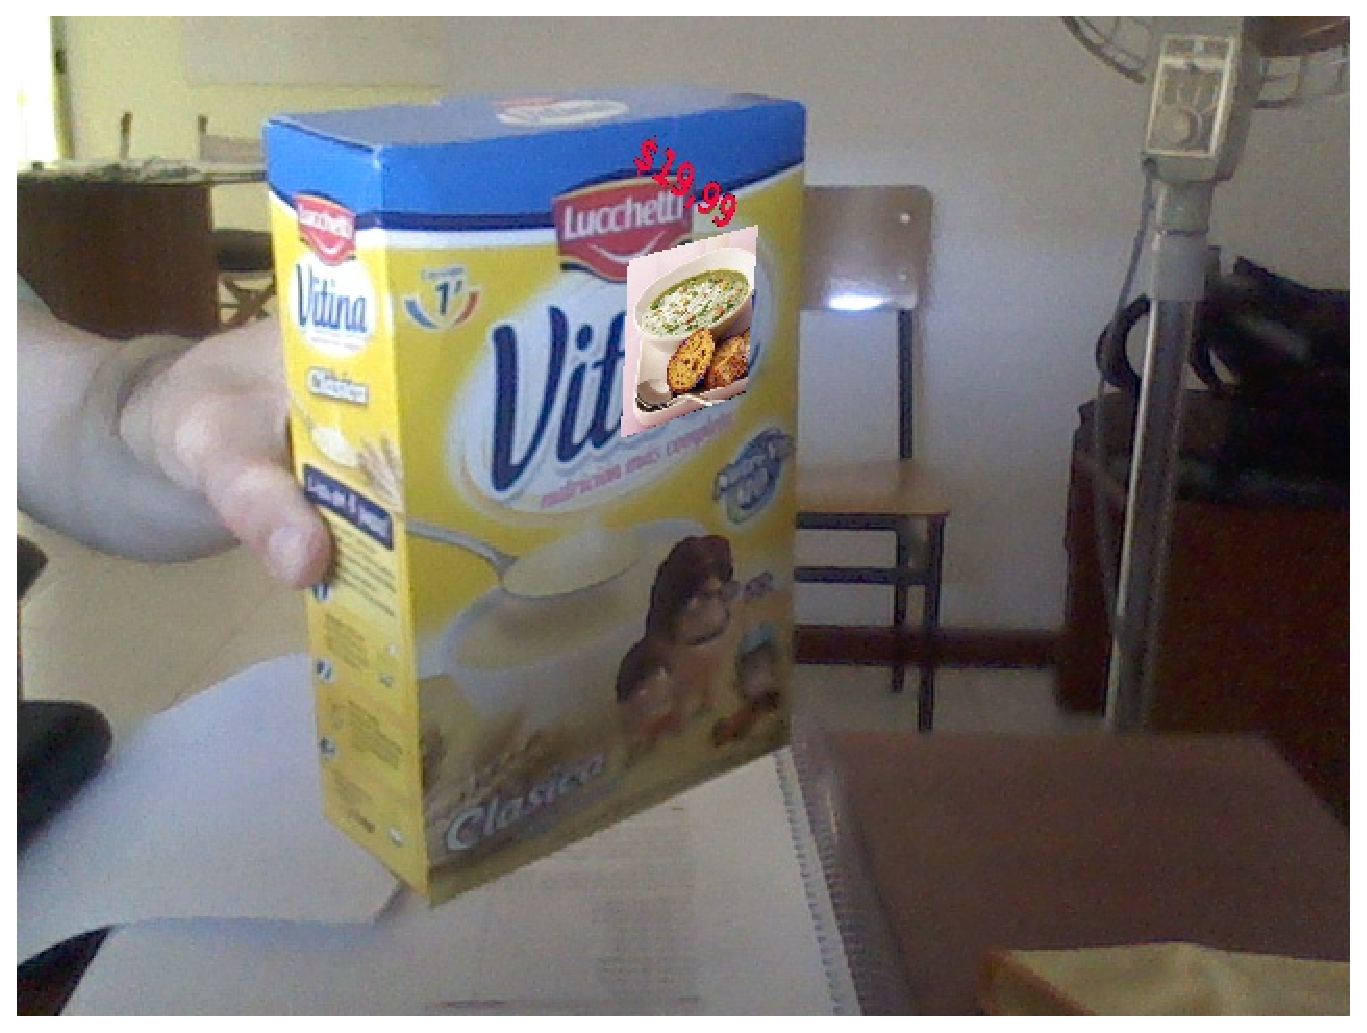
\includegraphics[width=2.5in]{../imgvitina/captured151,000000}}
\subfloat[][]{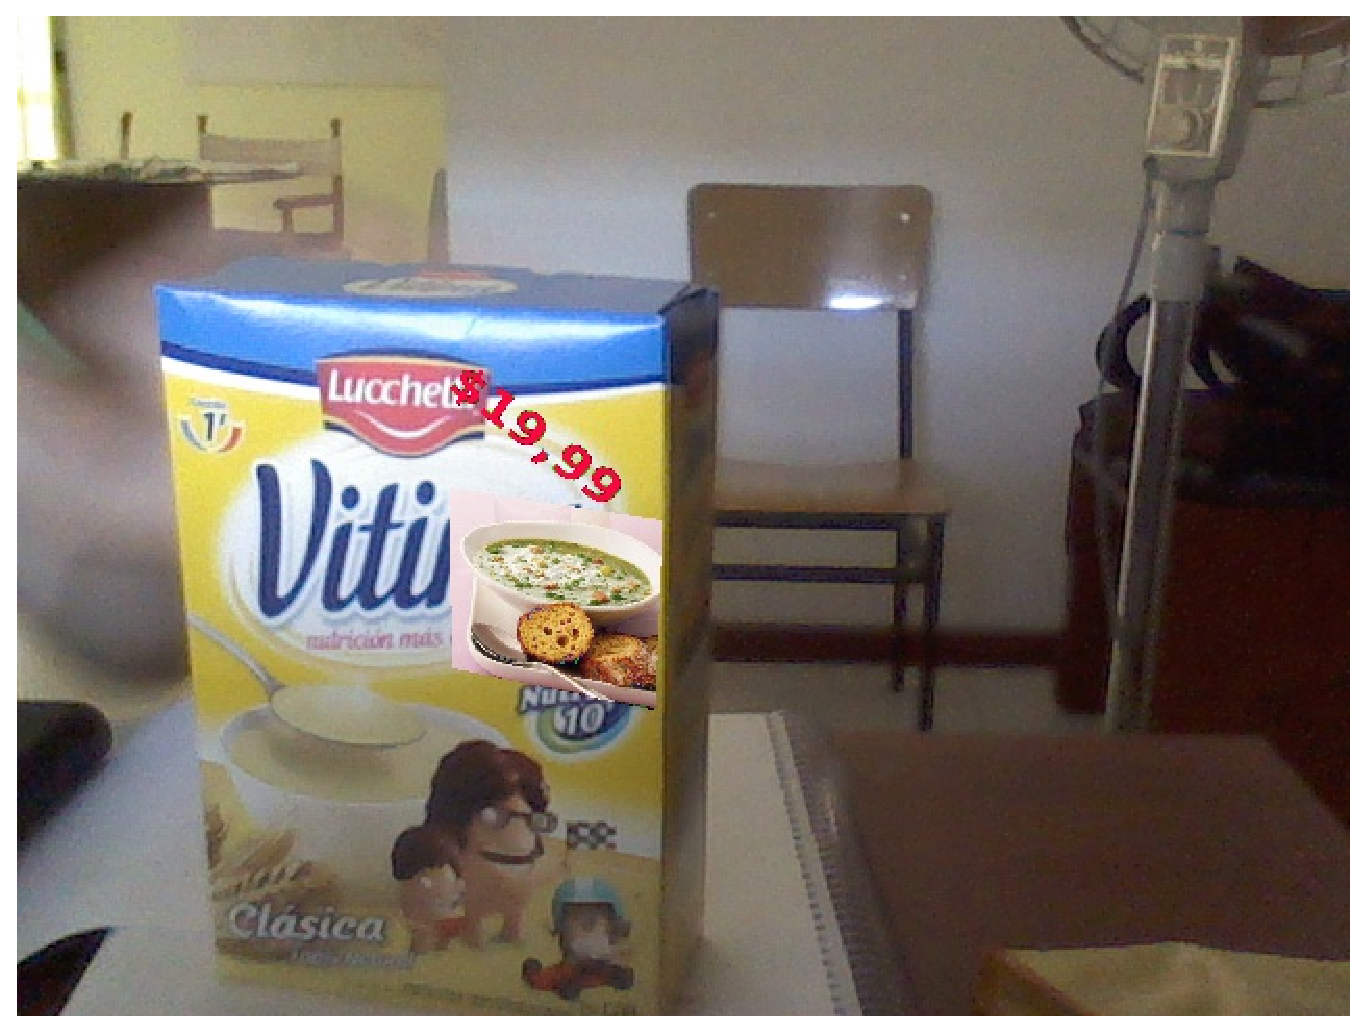
\includegraphics[width=2.5in]{../imgvitina/captured176,000000}\label{fig:last_detect_prototipo}}
\caption[Capturas en la etapa de ejecución para el prototipo publicitario]{Imagen patrón, objeto de realidad aumentada a sobreimprimir en el flujo de video y diferentes capturas en la etapa de ejecución para el prototipo publicitario.}
\label{fig:ejemplos_protitipos}
\end{figure}